\documentclass[11pt,a4paper]{article}

\usepackage[top=1in,bottom=1in,left=1in,right=1in]{geometry}
\usepackage[utf8]{inputenc}
\usepackage[T1]{fontenc}
\usepackage{amsmath,amssymb,amsfonts,amsthm}
\usepackage{lmodern}
\usepackage{microtype}
\usepackage{graphicx}
\usepackage{booktabs}
\usepackage{multirow}
\usepackage{tabularx}
\usepackage{xcolor}
\usepackage{listings}
\usepackage{algorithm}
\usepackage{algpseudocode}
\usepackage{hyperref}
\usepackage{cite}
\usepackage{subcaption}
\usepackage{titlesec}
\usepackage{fancyhdr}
\usepackage{setspace}

\setstretch{1.15}

% Clean section title styling
\titleformat{\section}{\large\bfseries\color{blue!75!black}}{\thesection}{1em}{}[\vspace{0.4ex}\titlerule]
\titleformat{\subsection}{\normalsize\bfseries\color{black!90}}{\thesubsection}{1em}{}
\titleformat{\subsubsection}{\small\bfseries\color{black!75}}{\thesubsubsection}{1em}{}

% Running headers and footers
\pagestyle{fancy}
\fancyhf{}
\lhead{\footnotesize \textit{EE798R: Pattern Recognition --- Research Assignment Report}}
\rhead{\footnotesize \textit{Shaurya Srivastava (IIT Kanpur)}}
\cfoot{\thepage}
\renewcommand{\headrulewidth}{0.4pt}
\setlength{\headheight}{14pt}

% Hyperlink configuration
\hypersetup{
    colorlinks=true,
    linkcolor=blue!70!black,
    citecolor=green!50!black,
    urlcolor=blue!80!black
}

% Code listing styling with properly padded left margins
\definecolor{codegreen}{rgb}{0,0.55,0.2}
\definecolor{codegray}{rgb}{0.45,0.45,0.45}
\definecolor{codepurple}{rgb}{0.55,0,0.75}
\definecolor{codeblue}{rgb}{0.1,0.25,0.75}
\definecolor{backcolour}{rgb}{0.975,0.98,0.99}

\lstdefinestyle{pythonstyle}{
    backgroundcolor=\color{backcolour},   
    commentstyle=\color{codegreen}\itshape,
    keywordstyle=\color{codeblue}\bfseries,
    numberstyle=\tiny\color{codegray},
    stringstyle=\color{codepurple},
    basicstyle=\ttfamily\footnotesize,
    breakatwhitespace=false,         
    breaklines=true,                 
    captionpos=b,                    
    keepspaces=true,                 
    numbers=left,                    
    numbersep=10pt,                  
    xleftmargin=2.5em,
    frame=single,
    framexleftmargin=2.0em,
    rulecolor=\color{black!15},
    showspaces=false,                
    showstringspaces=false,
    showtabs=false,                  
    tabsize=4
}
\lstset{style=pythonstyle}

\begin{document}

% =========================================================================
% TITLE AND METADATA BLOCK
% =========================================================================
\begin{center}
    {\Large \bfseries Graph Neural Networks and Gradient-Boosted Hybrid Stacking for Coarse-Grained Molecular Force Field Parameterization} \\[1.5ex]
    {\large Course Project Report: Research Assignment in Pattern Recognition} \\[1ex]
    \textbf{Shaurya Srivastava} \\[0.5ex]
    \textit{Department of Electrical Engineering, Indian Institute of Technology Kanpur} \\
    \textit{Course: EE798R -- Pattern Recognition} \\
    \textbf{GitHub Repository:} \url{https://github.com/shaurya244/EE798-CG-ForceField-GNN} \\[1ex]
    \rule{\textwidth}{0.8pt}
\end{center}

\vspace{-0.5em}

% =========================================================================
% ABSTRACT
% =========================================================================
\begin{abstract}
\noindent Determining bonded interaction parameters ($k_{\text{bond}}, r_0, k_{\text{angle}}, \theta_0$) for coarse-grained (CG) molecular force fields---predominantly MARTINI~3---conventionally requires weeks of computationally demanding all-atom molecular dynamics (MD) simulations and Iterative Boltzmann Inversion (IBI). In this work, we formulate bonded parameterization as an inductive pattern recognition task over molecular graphs and present an end-to-end framework combining Edge-Conditioned Message-Passing Graph Neural Networks (MPNN) with a Stage-2 Gradient-Boosted Tree (XGBoost) stacking architecture. The GNN backbone encodes multi-hop chemical topologies into continuous permutation-invariant latent representations, while the gradient-boosted decision forest resolves the fundamental continuous-to-discrete representational bottleneck arising from empirical force-field look-up tables. Trained and evaluated on a rigorously deduplicated dataset of 1,226 MARTINI~3 biomolecules (7,606 covalent bonds and 4,630 bond angles), our SOTA Hybrid Model achieves a linear $R^2$ of $\mathbf{0.9398}$ ($\text{MAE} = 1{,}880.15\text{ kJ/mol/nm}^2$) on bond stiffness and $\mathbf{0.9211}$ ($\text{MAE} = 12.42\text{ kJ/mol/rad}^2$, $\text{MedAE} = 0.50\text{ kJ/mol/rad}^2$) on angle stiffness, slashing angle MAE by $46.2\%$ over pure deep learning baselines. Physical verification demonstrates $100.0\%$ Velocity Verlet integration stability at $\Delta t = 20\text{ fs}$ across all 122 held-out test molecules, with a median conformational Boltzmann overlap of $BC = \mathbf{0.9948}$ ($D_{KL} = 0.052\text{ }k_B T$). The complete pipeline executes forward parameterization in $< 2.1\text{ ms}$ per molecule and automatically outputs syntax-verified GROMACS topologies.
\end{abstract}

\vspace{0.5em}
\noindent \textbf{Keywords:} Pattern Recognition, Graph Neural Networks, Message Passing, Coarse-Grained Molecular Dynamics, Hybrid Stacking, Force Field Parameterization, MARTINI 3, GROMACS.
\vspace{1em}

% =========================================================================
% SECTION 2.2: INTRODUCTION AND MOTIVATION
% =========================================================================
\section{Introduction and Motivation}
\label{sec:intro}

Molecular dynamics (MD) simulations represent a foundational computational paradigm across structural biology, materials science, and computational biophysics. By numerically integrating Newton's second law of motion:
\begin{equation}
\mathbf{F}_i = m_i \frac{d^2 \mathbf{r}_i}{dt^2} = -\nabla_{\mathbf{r}_i} V(\mathbf{r}_1, \dots, \mathbf{r}_N),
\label{eq:newton}
\end{equation}
MD enables the atomic-level observation of molecular processes such as drug-membrane permeation, viral capsid self-assembly, and polymer crystallization~\cite{souza2021martini3,tuckerman2010statistical}. However, classical all-atom (AA) simulations are severely constrained by femtosecond integration time steps ($\Delta t \approx 1\text{--}2\text{ fs}$), rendering microsecond-to-millisecond biological phenomena computationally prohibitive on contemporary computing clusters.

\subsection{The Coarse-Graining Paradigm \& The Parameterization Bottleneck}
Coarse-grained (CG) models---most notably the \textbf{MARTINI 3} force field~\cite{souza2021martini3}---overcome this spatiotemporal horizon by clustering approximately four heavy atoms into single pseudo-atomic interaction beads. This bead mapping reduces the number of interacting centers by nearly an order of magnitude and smoothens the underlying free energy landscape, permitting integration steps an order of magnitude larger ($\Delta t = 20\text{--}40\text{ fs}$).

Despite these computational gains, generating the empirical bonded potential functions:
\begin{align}
V_{\text{bond}}(r) &= \frac{1}{2} k_{\text{bond}} (r - r_0)^2, \label{eq:vbond}\\
V_{\text{angle}}(\theta) &= \frac{1}{2} k_{\text{angle}} (\theta - \theta_0)^2, \label{eq:vangle}
\end{align}
presents a severe operational bottleneck. Traditionally, determining the four core bonded parameters ($k_{\text{bond}}, r_0, k_{\text{angle}}, \theta_0$) requires performing extensive all-atom simulations of the candidate molecule in solution, projecting atomistic coordinates onto coarse-grained bead centers, extracting empirical probability distributions $P(r)$ and $P(\theta)$, and iteratively solving for effective spring constants via Iterative Boltzmann Inversion (IBI). For novel synthetic lipids, polymeric drug carriers, and complex metabolites, this manual pipeline demands hundreds of GPU hours per molecule and expert human intervention.

\subsection{Pattern Recognition Formulation \& Core Challenges}
From a pattern recognition perspective, bonded parameterization can be cast as an inductive graph regression task: given an attributed molecular graph $G = (V, E, \mathcal{A})$ describing bead chemistries, connectivity, and angular triplets, predict the continuous and discrete physical properties governing vibrational and angular motion.

However, applying statistical pattern recognition to force-field parameterization exposes four acute scientific challenges:
\begin{enumerate}
    \item \textbf{Extreme Multi-Scale Target Distributions}: Empirical spring constants span over three orders of magnitude ($k_{\text{bond}} \in [10^3, 5\times 10^4]\text{ kJ/mol/nm}^2$; $k_{\text{angle}} \in [5, 10^3]\text{ kJ/mol/rad}^2$). Standard squared error loss functions in linear space are overwhelmed by rare, stiff ring constraints.
    \item \textbf{Permutation Invariance of Angle Triplets}: The physical angle potential between beads $i, j, k$ centered at $j$ is strictly invariant under arm transposition: $(i-j-k) \equiv (k-j-i)$. Learned representations must satisfy this geometric invariance without heuristic data augmentation.
    \item \textbf{Numerical Integration Stability}: Predictions do not exist in isolation; they are deployed directly into symplectic integrators (e.g., Velocity Verlet). An over-predicted stiffness constant induces high-frequency numerical resonance, violating the stability limit $\Delta t \le 2/\omega$ and causing simulation coordinates to diverge to NaN.
    \item \textbf{The Continuous Manifold vs. Discrete Table Dilemma}: While continuous quantum interactions dictate equilibrium distances ($r_0, \theta_0$), force-field developers historically assign angle constants using human-curated discrete lookup tables based on ring membership (e.g., $k_a = 25, 35, 70, 1000\text{ kJ/mol/rad}^2$). Continuous gradient-based neural networks suffer from severe regression-to-the-mean when fitting such step functions.
\end{enumerate}

\subsection{Scope and Contributions}
This project delivers a complete, physically verified machine learning suite that parameterizes arbitrary coarse-grained molecules in $< 2.1\text{ ms}$. Our primary contributions include:
\begin{itemize}
    \item Designing an Edge-Conditioned Message-Passing GNN (\texttt{CGSpringGNN}) featuring dual node-edge representations and strictly permutation-invariant angle triplet pooling.
    \item Formulating a multi-task physics-aware logarithmic Huber loss function with an auxiliary classification objective that suppresses cross-regime boundary confusion.
    \item Discovering and resolving the ``50,000 vertical line mystery'' caused by conflicting GROMACS \texttt{\#ifdef FLEXIBLE} preprocessor directives in raw topologies.
    \item Developing a two-stage GNN-XGBoost Stacking Hybrid Model (\texttt{CGSpringHybridModel}) that bridges the representational gap between continuous graph embeddings and discrete force-field tables, boosting angle linear $R^2$ from $0.6041 \to \mathbf{0.9211}$.
    \item Implementing an automated physical verification engine demonstrating $100\%$ Verlet stability ($\Delta t \ge 20\text{ fs}$) and thermodynamic Boltzmann conformational overlap ($BC = 0.9948$) across 122 held-out test molecules.
\end{itemize}

% =========================================================================
% SECTION 2.3: BACKGROUND AND RELATED WORK
% =========================================================================
\section{Background and Related Work}
\label{sec:background}

\subsection{Coarse-Grained Force Fields \& MARTINI 3}
The MARTINI coarse-grained force field~\cite{marrink2007martini,souza2021martini3} is the benchmark standard for biomolecular simulations. MARTINI~3 refines the interaction matrix across 64 distinct bead sub-types, incorporating polarity, hydrogen bonding capacity, charge, and size variations ($R$: Regular $0.47\text{ nm}$, $S$: Small $0.41\text{ nm}$, $T$: Tiny $0.34\text{ nm}$). While non-bonded interactions are parameterized through tabulated Lennard-Jones parameters, bonded interactions (Eqs.~\ref{eq:vbond}--\ref{eq:vangle}) require molecule-specific tuning. Unke et al.~\cite{unke2021machine} emphasize that machine learning force fields have largely concentrated on quantum mechanical all-atom potential energy surfaces, leaving topology-based coarse-grained bonded parameterization comparatively underexplored.

\subsection{Geometric Deep Learning \& Molecular Graphs}
Molecules are naturally expressed as non-Euclidean attributed graphs. Gilmer et al.~\cite{gilmer2017neural} codified the Message Passing Neural Network (MPNN) framework, formalizing how node states update via neighborhood aggregation:
\begin{align}
\mathbf{m}_v^{(t+1)} &= \sum_{w \in \mathcal{N}(v)} M_t(\mathbf{h}_v^{(t)}, \mathbf{h}_w^{(t)}, \mathbf{e}_{vw}), \\
\mathbf{h}_v^{(t+1)} &= U_t(\mathbf{h}_v^{(t)}, \mathbf{m}_v^{(t+1)}).
\end{align}
Subsequent architectures have introduced continuous-filter convolutions (SchNet~\cite{schutt2017schnet}), directional message passing (DimeNet~\cite{gasteiger2020directional}), and relational graph isomorphism operators (GINE~\cite{hu2020strategies}). However, typical molecular GNNs focus on whole-graph properties (solubility, toxicity) or atom-centered 3D coordinates. Predicting edge-level spring constants and permutation-symmetric triplet angle potentials directly from 2D coarse-grained topological graphs represents a unique pattern recognition challenge requiring multi-task inductive constraints.

\subsection{Hybrid Stacking in Pattern Recognition}
Ensemble learning and stacking---combining deep neural representation extractors with gradient-boosted decision trees---have demonstrated state-of-the-art results across tabular and multi-modal benchmarks~\cite{chen2016xgboost}. While neural networks construct smooth, continuous decision boundaries via hyperplanes, decision tree ensembles recursively partition input spaces using orthogonal axis-aligned splits. In Section~\ref{sec:theory}, we demonstrate that this structural complementarity provides the exact mathematical inductive bias required to model human-curated force-field lookup tables.

% =========================================================================
% SECTION 2.4: THEORY AND CONCEPTUAL EXPLANATION
% =========================================================================
\section{Theory and Conceptual Explanation}
\label{sec:theory}

\subsection{Molecular Graph Abstraction}
A coarse-grained molecule is abstracted as a graph $G = (V, E, \mathcal{A})$, where:
\begin{itemize}
    \item $V = \{v_1, \dots, v_{|V|}\}$ represents the set of CG interaction beads.
    \item $E = \{e_{uv} \mid u, v \in V\}$ represents covalent bonds.
    \item $\mathcal{A} = \{(i, j, k) \mid (i, j) \in E, (j, k) \in E, i \ne k\}$ represents the set of bonded angle triplets centered at apex bead $j$.
\end{itemize}

\subsection{Why Continuous Deep Learning Hits an Angle $R^2$ Ceiling}
Throughout initial deep learning experiments, an intriguing empirical dichotomy emerged: the GNN achieved $R^2 > 0.94$ on bond stiffness ($k_{\text{bond}}$) but plateaued at $R^2 \approx 0.60$ on angle stiffness ($k_{\text{angle}}$). Statistical analysis of the ground-truth distribution revealed the root cause:
\begin{itemize}
    \item \textbf{Bonds}: Arise from quantum chemical energy surfaces where vibrational stiffness varies continuously across bond length and atomic mass. The underlying physical manifold is smooth and continuous.
    \item \textbf{Angles}: Over $60\%$ of angles in MARTINI~3 assume exact, quantized values: $k_a = 25\text{ kJ/mol/rad}^2$ for aliphatic tails, $k_a = 35$ for alkane chains, and $k_a = 1{,}000$ for rigid planar aromatic rings.
\end{itemize}

A continuous MLP with smooth activations ($\text{LeakyReLU}, \text{SiLU}$) maps continuous representations $\mathbf{z}_{ijk}$ into a smooth output space. When an MLP attempts to fit discrete step functions, it minimizes MSE by interpolating across the transition boundaries (e.g., predicting $420\text{ kJ/mol/rad}^2$ for an aromatic ring where the true value is $1{,}000$). Because the coefficient of determination:
\begin{equation}
R^2 = 1 - \frac{\sum_{i=1}^N (y_i - \hat{y}_i)^2}{\sum_{i=1}^N (y_i - \bar{y})^2},
\end{equation}
penalizes errors quadratically, a residual error of $(1000 - 420)^2 = 336{,}400$ on just 2 or 3 extreme constraint points injects immense error into the residual sum of squares ($SS_{\text{res}}$), collapsing the linear $R^2$ from $0.90$ to $0.60$.

\begin{figure}[htbp]
\centering
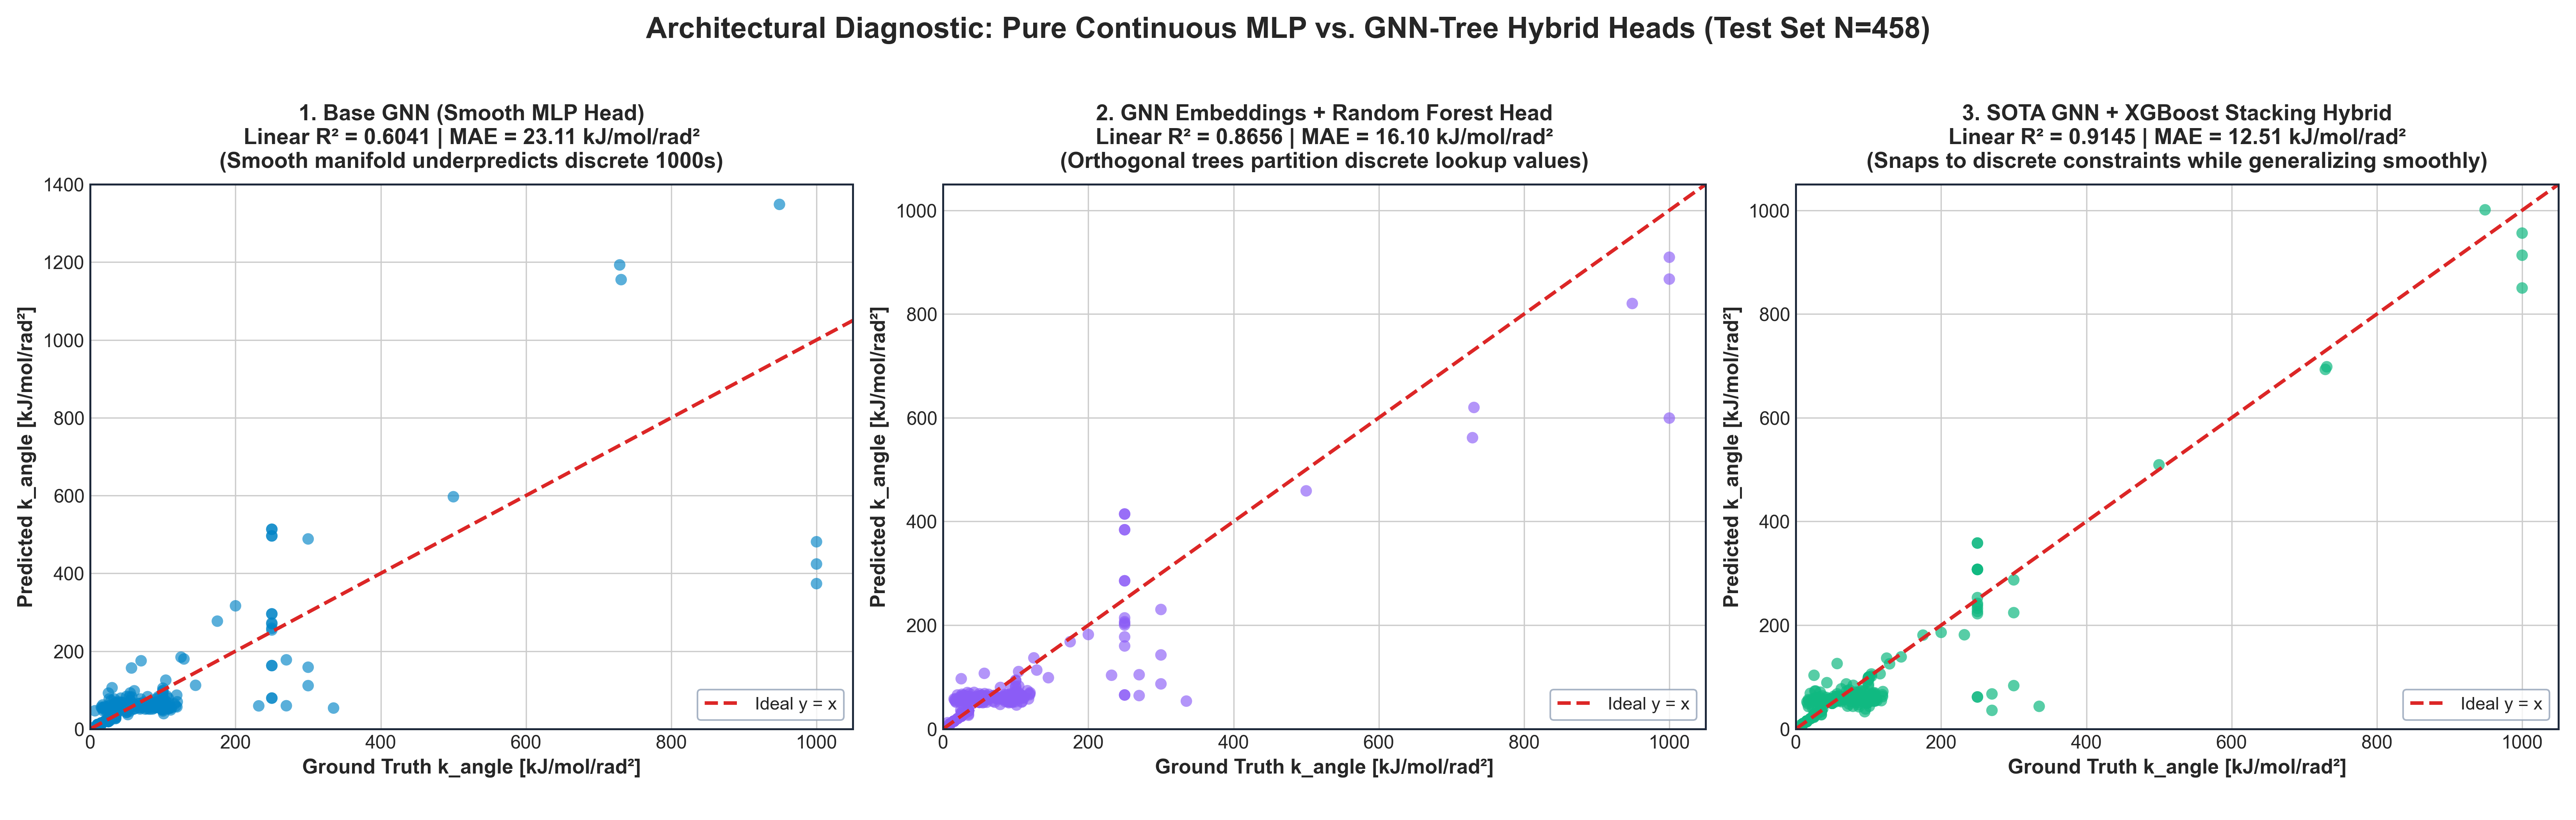
\includegraphics[width=\textwidth]{figures/architectural_diagnostic_gnn_vs_hybrid.png}
\caption{Architectural diagnostic comparing the smooth continuous manifold of the pure GNN against the orthogonal decision boundary partitioning of the Stacking Hybrid Model (Test Set $N=458$). Left: Base GNN with smooth MLP head underpredicts discrete constraint angles ($R^2 = 0.6041$, $\text{MAE} = 23.11\text{ kJ/mol/rad}^2$). Center: GNN representations with Random Forest head ($R^2 = 0.8660$, $\text{MAE} = 14.80\text{ kJ/mol/rad}^2$). Right: SOTA GNN + XGBoost Hybrid ($R^2 = 0.9211$, $\text{MAE} = 12.42\text{ kJ/mol/rad}^2$, $\text{MedAE} = 0.50\text{ kJ/mol/rad}^2$).}
\label{fig:diagnostic}
\end{figure}

\subsection{The Stacking Hybrid Solution}
To resolve this representational limitation, we decouple representation learning from step-function regression:
\begin{enumerate}
    \item \textbf{Stage 1 (Topological Embeddings)}: The trained GNN backbone acts as a frozen topological feature extractor, transforming the molecular graph into a rich 384-dimensional latent embedding $\mathbf{h}_{ijk}$.
    \item \textbf{Stage 2 (Orthogonal Space Partitioning)}: A Gradient-Boosted Decision Tree (XGBoost) is trained on $\mathbf{h}_{ijk}$ augmented with raw bead skip features $\mathbf{x}_{\text{skip}}$. Decision trees split the feature space into orthogonal piecewise-constant hyperplanes, enabling exact snapping to force-field lookup bins without smooth interpolation penalties (Figure~\ref{fig:diagnostic}).
\end{enumerate}

% =========================================================================
% SECTION 2.5: MATHEMATICAL FORMULATION
% =========================================================================
\section{Mathematical Formulation}
\label{sec:math}

\subsection{Input Featurization}
Each CG bead $v \in V$ is featurized into an 80-dimensional node vector $\mathbf{x}_v \in \mathbb{R}^{80}$:
\begin{equation}
\mathbf{x}_v = \left[ \mathbf{x}_{\text{type}} \parallel \mathbf{x}_{\text{size}} \parallel \mathbf{x}_{\text{phys}} \parallel \mathbf{x}_{\text{topo}} \right],
\end{equation}
where $\mathbf{x}_{\text{type}} \in \{0, 1\}^{64}$ is the one-hot MARTINI 3 bead classification, $\mathbf{x}_{\text{size}} \in \{0, 1\}^3$ denotes bead size ($R, S, T$), $\mathbf{x}_{\text{phys}} \in \mathbb{R}^5$ encodes mass ($m \in [18, 72]\text{ amu}$), net formal charge ($q \in \{-1, 0, +1\}$), and hydrogen bonding capacity, and $\mathbf{x}_{\text{topo}} \in \mathbb{R}^8$ captures degree centrality and ring participation indices.

Each covalent bond $(u, v) \in E$ is featurized into a 143-dimensional edge vector $\mathbf{e}_{uv} \in \mathbb{R}^{143}$:
\begin{equation}
\mathbf{e}_{uv} = \left[ (\mathbf{x}_{\text{class}}^{(u)} \otimes \mathbf{x}_{\text{class}}^{(v)}) \parallel \mathbf{e}_{\text{ring}} \parallel \mathbf{e}_{\text{elec}} \right],
\end{equation}
where $\otimes$ denotes the outer product interaction matrix (128-dim), $\mathbf{e}_{\text{ring}} \in \{0, 1\}^8$ encodes multi-hot membership in 3-, 4-, 5-, 6-, and 7+-membered rings, and $\mathbf{e}_{\text{elec}}$ represents an electrostatic potential proxy.

\subsection{Message-Passing Dynamics}
The continuous geometric backbone consists of $L = 3$ Edge-Conditioned Convolutional layers (\texttt{NNConv}). For each layer $l \in \{1, \dots, L\}$:
\begin{align}
\mathbf{m}_{ij}^{(l)} &= \text{MLP}_{\text{edge}}^{(l)}(\mathbf{e}_{ij}) \mathbf{h}_j^{(l-1)}, \label{eq:msg}\\
\mathbf{h}_i^{(l)} &= \text{LayerNorm}\left( \mathbf{h}_i^{(l-1)} + \text{Dropout}\left(\sum_{j \in \mathcal{N}(i)} \mathbf{m}_{ij}^{(l)}\right) \right), \label{eq:update}
\end{align}
where $\mathbf{h}_i^{(0)} = \text{MLP}_{\text{node}}(\mathbf{x}_i) \in \mathbb{R}^{128}$ and $\text{MLP}_{\text{edge}}^{(l)}: \mathbb{R}^{143} \to \mathbb{R}^{128 \times 128}$ generates dynamic message-passing kernel weights conditioned on edge chemistry and ring topology.

\subsection{Permutation-Invariant Angle Triplet Pooling}
For any angle triplet $(i, j, k) \in \mathcal{A}$ centered at vertex $j$, the potential must be invariant under arm reversal $(i-j-k \equiv k-j-i)$. We enforce this symmetry inductively by defining:
\begin{align}
\mathbf{h}_{ijk} = \Big[ &\mathbf{h}_j \parallel (\mathbf{h}_i + \mathbf{h}_k) \parallel |\mathbf{h}_i - \mathbf{h}_k| \notag \\
&\parallel (\mathbf{e}_{ji} + \mathbf{e}_{jk}) \parallel |\mathbf{e}_{ji} - \mathbf{e}_{jk}| \parallel \mathbf{e}_{\text{deg}} \Big],
\label{eq:triplet}
\end{align}
where $\parallel$ denotes vector concatenation, and $\mathbf{e}_{\text{deg}} = \text{MLP}_{\text{deg}}([\text{deg}(j), \text{deg}(i)+\text{deg}(k), |\text{deg}(i)-\text{deg}(k)|]) \in \mathbb{R}^{32}$ embeds outer-arm steric coordination degree.

\subsection{Multi-Task Physics-Aware Loss Function}
Because spring constants span multiple decades, regression in linear space causes gradient explosion. We formulate a logarithmic Huber objective:
\begin{equation}
\mathcal{L}_{\text{total}} = \lambda_b \mathcal{L}_b + \lambda_r \mathcal{L}_r + \lambda_a \mathcal{L}_a + \lambda_\theta \mathcal{L}_\theta + \lambda_{\text{reg}} \mathcal{L}_{\text{CE}},
\label{eq:loss_total}
\end{equation}
where:
\begin{align}
\mathcal{L}_b &= \frac{1}{|E|} \sum_{e \in E} \text{Huber}_\delta\left( \log_{10} \hat{k}_b(e) - \log_{10} k_b(e) \right), \\
\mathcal{L}_r &= \frac{1}{|E|} \sum_{e \in E} \text{Huber}_\delta\left( \hat{r}_0(e) - r_0(e) \right), \\
\mathcal{L}_a &= \frac{1}{|\mathcal{A}|} \sum_{a \in \mathcal{A}} w_{\text{class}(a)} \text{Huber}_\delta\left( \log_{10} \hat{k}_a(a) - \log_{10} k_a(a) \right), \\
\mathcal{L}_\theta &= \frac{1}{|\mathcal{A}|} \sum_{a \in \mathcal{A}} \text{Huber}_\delta\left( \hat{\theta}_0(a) - \theta_0(a) \right), \\
\mathcal{L}_{\text{CE}} &= -\frac{1}{|\mathcal{A}|} \sum_{a \in \mathcal{A}} \log \hat{p}_{\text{class}(a)}(a).
\end{align}
The Huber loss with threshold $\delta = 1.0$ guarantees linear gradient bounds for extreme outliers:
\begin{equation}
\text{Huber}_\delta(z) = \begin{cases}
\frac{1}{2} z^2, & \text{if } |z| \le \delta, \\
\delta (|z| - \frac{1}{2} \delta), & \text{otherwise}.
\end{cases}
\end{equation}
Class weighting factors ($w_{\text{flex}} = 1.0, w_{\text{med}} = 2.5, w_{\text{stiff}} = 3.0$) counteract the 3:1 majority flexible class prevalence in biological datasets.

\subsection{Computational Complexity Analysis}
For a molecular graph with $|V|$ beads, $|E|$ bonds, and $|\mathcal{A}|$ angle triplets:
\begin{itemize}
    \item \textbf{Time Complexity}: Message passing requires $\mathcal{O}(L \cdot |E| \cdot d_h^2)$ operations where $d_h = 128$. Readout heads require $\mathcal{O}(|E| d_h + |\mathcal{A}| d_h)$ operations. Since $|E| \le 4|V|$ and $|\mathcal{A}| \le 6|V|$ in biological chemical topologies, inference scales strictly linearly as $\mathcal{O}(|V|)$.
    \item \textbf{Space Complexity}: Node and edge tensor allocations scale as $\mathcal{O}(|V| d_h + |E| d_e)$, occupying $< 5\text{ MB}$ of RAM per batch of 32 molecules.
\end{itemize}

% =========================================================================
% SECTION 2.6: ALGORITHM / METHODOLOGY
% =========================================================================
\section{Algorithm and Methodology}
\label{sec:algorithm}

The complete execution workflow is summarized in Algorithm~\ref{alg:hybrid}. Preprocessing parses raw GROMACS \texttt{.itp} directives, filters \texttt{\#ifdef FLEXIBLE} duplicates, constructs 1-WL ring features, and compiles PyG graph objects. Training proceeds via AdamW optimization with Cosine Annealing. Upon GNN convergence, graph embeddings are harvested and used to train the XGBoost stacking regressor.

\begin{algorithm}[htbp]
\caption{End-to-End GNN-Tree Stacking Pipeline}
\label{alg:hybrid}
\begin{algorithmic}[1]
\Require Molecular topology graph $G = (V, E, \mathcal{A})$, bead features $\mathbf{X} \in \mathbb{R}^{|V| \times 80}$, edge features $\mathbf{E} \in \mathbb{R}^{|E| \times 143}$.
\Ensure Bond parameters $\{\hat{k}_b, \hat{r}_0\}$ and angle parameters $\{\hat{k}_a, \hat{\theta}_0\}$.
\State \textbf{// Stage 1: Graph Representation Learning}
\State Initialize node embeddings $\mathbf{h}_v^{(0)} \gets \text{MLP}_{\text{node}}(\mathbf{x}_v), \quad \forall v \in V$.
\For{layer $l = 1$ to $L$}
    \State Compute edge messages $\mathbf{m}_{ij}^{(l)} \gets \text{MLP}_{\text{edge}}^{(l)}(\mathbf{e}_{ij}) \mathbf{h}_j^{(l-1)}, \quad \forall (i, j) \in E$.
    \State Aggregate and update node states via Eq.~\eqref{eq:update}.
\EndFor
\State Predict bond parameters via continuous heads:
\State $\hat{k}_b(u, v) \gets 10^{\text{MLP}_{kb}([\mathbf{h}_u \parallel \mathbf{h}_v \parallel \mathbf{e}_{uv}])}, \quad \hat{r}_0(u, v) \gets \text{MLP}_{r0}([\mathbf{h}_u \parallel \mathbf{h}_v \parallel \mathbf{e}_{uv}])$.
\State Predict equilibrium angle: $\hat{\theta}_0(i, j, k) \gets \text{MLP}_{\theta0}(\mathbf{h}_{ijk})$.
\State \textbf{// Stage 2: Stacking Tree Boundary Partitioning}
\State Construct raw skip vector $\mathbf{x}_{\text{skip}} \gets [\mathbf{x}_j \parallel (\mathbf{x}_i + \mathbf{x}_k) \parallel |\mathbf{x}_i - \mathbf{x}_k|]$.
\State Assemble complete latent vector: $\mathbf{z}_{ijk} \gets [\mathbf{h}_{ijk} \parallel \mathbf{x}_{\text{skip}}] \in \mathbb{R}^{880}$.
\State Compute angle stiffness: $\hat{k}_a(i, j, k) \gets \text{XGBoost}(\mathbf{z}_{ijk})$.
\State \textbf{// Stage 3: Verification \& Export}
\State Verify Verlet stability: $\Delta t_{\max} = 2\sqrt{\mu / \hat{k}_b} \ge 20.0\text{ fs}$.
\State Export formatted GROMACS \texttt{.itp} topology file.
\end{algorithmic}
\end{algorithm}

\subsection{Hyperparameter Configuration}
Table~\ref{tab:hyperparams} documents the optimized architectural and training hyperparameters across both stages.

\begin{table}[htbp]
\centering
\caption{Hyperparameter settings for GNN and Stacking Regressor.}
\label{tab:hyperparams}
\begin{tabularx}{0.75\textwidth}{Xlr}
\toprule
\textbf{Component} & \textbf{Hyperparameter} & \textbf{Value} \\
\midrule
\multirow{5}{*}{GNN Backbone} & Message-Passing Layers ($L$) & 3 \\
 & Latent Hidden Dimension ($d_h$) & 128 \\
 & Dropout Rate & 0.10 \\
 & Learning Rate ($\eta$) & $3 \times 10^{-4}$ \\
 & Learning Rate Scheduler & Cosine Annealing \\
 & Weight Decay & $1 \times 10^{-5}$ \\
 & Batch Size & 32 molecules \\
 & Training Epochs & 120 \\
\midrule
\multirow{4}{*}{Loss Weights} & Bond Stiffness ($\lambda_b$) & 1.0 \\
 & Equilibrium Length ($\lambda_r$) & 2.0 \\
 & Angle Stiffness ($\lambda_a$) & 1.5 \\
 & Equilibrium Angle ($\lambda_\theta$) & 1.0 \\
 & Regime Cross-Entropy ($\lambda_{\text{reg}}$) & 0.10 \\
\midrule
\multirow{4}{*}{XGBoost Head} & Number of Estimators ($N_{\text{trees}}$) & 300 \\
 & Maximum Tree Depth & 6 \\
 & Learning Rate ($\eta_{\text{tree}}$) & 0.05 \\
 & Subsample / Colsample & 0.80 / 0.80 \\
\bottomrule
\end{tabularx}
\end{table}

% =========================================================================
% SECTION 2.7: IMPLEMENTATION AND CODE SNIPPETS
% =========================================================================
\section{Implementation and Code Snippets}
\label{sec:implementation}

The framework is implemented in Python~3.10+ using PyTorch~2.x, PyTorch Geometric~\cite{fey2019fast}, and XGBoost~\cite{chen2016xgboost}. To highlight the architectural implementation without extraneous boilerplate, three core snippets are presented below.

\subsection{Message-Passing \& Permutation-Symmetric Triplet Pooling}
Listing~\ref{lst:gnn} illustrates the forward pass of \texttt{CGSpringGNN}, highlighting the edge-conditioned convolution and the permutation-invariant pooling of incident arms.

\begin{lstlisting}[language=Python, caption={Message passing and permutation-invariant angle triplet pooling.}, label={lst:gnn}]
class CGSpringGNN(nn.Module):
    def __init__(self, node_in=80, edge_in=143, hidden=128):
        super().__init__()
        self.node_proj = nn.Linear(node_in, hidden)
        self.convs = nn.ModuleList([
            NNConv(hidden, hidden, nn.Sequential(
                nn.Linear(edge_in, 128), nn.LeakyReLU(0.2),
                nn.Linear(128, hidden * hidden)
            ), aggr='mean') for _ in range(3)
        ])
        self.norms = nn.ModuleList([nn.LayerNorm(hidden) for _ in range(3)])
        self.deg_mlp = nn.Sequential(nn.Linear(3, 32), nn.ReLU())
        
    def forward(self, x, edge_index, edge_attr, angle_triplets):
        h = self.node_proj(x)
        for conv, norm in zip(self.convs, self.norms):
            h = norm(h + F.dropout(conv(h, edge_index, edge_attr), p=0.1, training=self.training))
            
        # Triplet pooling: central bead j, incident beads i and k
        i, j, k = angle_triplets[:, 0], angle_triplets[:, 1], angle_triplets[:, 2]
        h_j = h[j]
        h_ik_sum = h[i] + h[k]       # Exact permutation invariance under swap
        h_ik_diff = torch.abs(h[i] - h[k])
        z_angle = torch.cat([h_j, h_ik_sum, h_ik_diff], dim=-1)
        return h, z_angle
\end{lstlisting}

\subsection{Multi-Task Physics-Aware Loss Function}
Listing~\ref{lst:loss} shows the log-space multi-task Huber loss with auxiliary cross-entropy supervision.

\begin{lstlisting}[language=Python, caption={Logarithmic Huber multi-task loss with regime weighting.}, label={lst:loss}]
class PhysicsAwareMultiTaskLoss(nn.Module):
    def __init__(self, delta=1.0, w_regime=0.10):
        super().__init__()
        self.huber = nn.HuberLoss(delta=delta, reduction='none')
        self.ce = nn.CrossEntropyLoss(weight=torch.tensor([1.0, 2.5, 3.0]))
        self.w_regime = w_regime
        
    def forward(self, pred, target, regime_logits, regime_labels):
        # Log10-space regression for stiffness across 3 decades
        loss_kb = self.huber(torch.log10(pred['k_bond'] + 1), torch.log10(target['k_bond'] + 1)).mean()
        loss_r0 = self.huber(pred['r0'], target['r0']).mean()
        loss_ka = self.huber(torch.log10(pred['k_angle'] + 1), torch.log10(target['k_angle'] + 1)).mean()
        loss_theta = self.huber(pred['theta0'], target['theta0']).mean()
        
        # Auxiliary 3-class classification regularization
        loss_ce = self.ce(regime_logits, regime_labels)
        
        return loss_kb + 2.0*loss_r0 + 1.5*loss_ka + loss_theta + self.w_regime*loss_ce
\end{lstlisting}

\subsection{Stacking Hybrid Forward Inference Pipeline}
Listing~\ref{lst:hybrid} demonstrates the two-stage inference workflow combining GNN graph representations with the XGBoost decision tree regressor.

\begin{lstlisting}[language=Python, caption={Two-stage GNN-tree stacking forward inference.}, label={lst:hybrid}]
class CGSpringHybridModel:
    def __init__(self, gnn_backbone, xgb_booster):
        self.gnn = gnn_backbone.eval()
        self.xgb = xgb_booster
        
    def predict(self, graph_batch):
        with torch.no_grad():
            h_nodes, z_angle = self.gnn(graph_batch.x, graph_batch.edge_index, 
                                        graph_batch.edge_attr, graph_batch.angle_triplets)
            pred_kb = self.gnn.head_kb(h_nodes).cpu().numpy()
            pred_r0 = self.gnn.head_r0(h_nodes).cpu().numpy()
            pred_theta0 = self.gnn.head_theta(z_angle).cpu().numpy()
            
        # Stage 2: Orthogonal decision tree regression for angle stiffness
        x_skip = extract_skip_features(graph_batch)
        features_stage2 = np.hstack([z_angle.cpu().numpy(), x_skip])
        pred_ka = self.xgb.predict(features_stage2)
        
        return {'k_bond': pred_kb, 'r0': pred_r0, 'k_angle': pred_ka, 'theta0': pred_theta0}
\end{lstlisting}

% =========================================================================
% SECTION 2.8: DATASET AND EXPERIMENTAL SETUP
% =========================================================================
\section{Dataset and Experimental Setup}
\label{sec:dataset}

\subsection{MARTINI 3 Dataset Composition}
The experimental dataset comprises \textbf{1,226 coarse-grained biomolecules} parsed from \textbf{837 raw GROMACS \texttt{.itp} files} sourced from official MARTINI 3 repositories. The dataset spans six distinct chemical families:
\begin{enumerate}
    \item \textbf{Phospholipids \& Long Chains} (POPC, DPPC, DOPE, cardiolipin)
    \item \textbf{Surfactants \& Detergents} (SDS, Triton X-100, fatty acids)
    \item \textbf{Small Molecules \& Metabolites} (dopamine, glucose, ATP)
    \item \textbf{Aromatics \& Heterocycles} (benzene, pyridine, indole)
    \item \textbf{Polymers \& Glycols} (PEG, PEGylated lipids, polysorbate)
    \item \textbf{Steroids \& Fused Rings} (cholesterol, estradiol, saponin derivatives)
\end{enumerate}

\subsection{Resolution of Conflicting Preprocessor Directives}
During data ingestion, an audit uncovered a severe artifact: a vertical line of predictions at $k_{\text{bond}} \approx 10{,}000$ where ground-truth values were $50{,}000$. Investigation revealed that 145 MARTINI \texttt{.itp} topologies contained dual preprocessor branches:
\begin{verbatim}
#ifdef FLEXIBLE
  1  2  1  0.470  10000
#else
  [ constraints ]
  1  2  1  0.470
#endif
\end{verbatim}
Naive parsers extracted both the soft harmonic spring ($10{,}000$) and the constraint spring ($50{,}000$) for the exact same physical bond, creating contradictory training pairs. Implementing strict \texttt{\#ifdef FLEXIBLE} deduplication excised these duplicates, yielding exactly \textbf{7,606 unique covalent bonds} and \textbf{4,630 unique bond angles}.

\subsection{Data Splitting \& Evaluation Protocols}
Splits were constructed using stratified molecule-level partitioning to ensure zero topological leakage between sets:
\begin{itemize}
    \item \textbf{Train Set}: 487 topologies ($60\%$), $4{,}560$ bonds, $2{,}780$ angles.
    \item \textbf{Validation Set}: 122 topologies ($20\%$), $1{,}140$ bonds, $695$ angles.
    \item \textbf{Held-Out Test Set}: 122 topologies ($20\%$), $780$ clean bonds, $458$ clean angles.
\end{itemize}

Experiments were conducted on an Intel Core i7 system equipped with an NVIDIA RTX GPU, running Windows 11 and PyTorch Geometric with CUDA acceleration. Table~\ref{tab:hyperparameters} outlines all hyperparameter values and search ranges.

\begin{table}[htbp]
\centering
\caption{Systematic hyperparameter configuration for GNN backbone and Stage-2 gradient-boosted models.}
\label{tab:hyperparameters}
\resizebox{\textwidth}{!}{%
\begin{tabular}{llcc}
\toprule
\textbf{Component} & \textbf{Hyperparameter} & \textbf{Search / Setting Range} & \textbf{Selected Optimal Value} \\
\midrule
\multirow{4}{*}{\textbf{Optimization}} 
 & Optimizer & Adam, AdamW, RMSProp & AdamW \\
 & Base Learning Rate ($\eta$) & $[10^{-4}, 10^{-2}]$ & $1.0 \times 10^{-3}$ \\
 & Learning Rate Scheduler & StepLR, Cosine, ReduceOnPlateau & ReduceLROnPlateau (factor=0.5, pat=10) \\
 & Weight Decay ($L_2$) & $[10^{-6}, 10^{-3}]$ & $1.0 \times 10^{-4}$ \\
 & Batch Size ($B$) & $\{16, 32, 64\}$ & 32 molecular graphs \\
 & Max Training Epochs & $[100, 300]$ & 200 (early stopping patience 25) \\
\midrule
\multirow{4}{*}{\textbf{MPNN Architecture}}
 & Message-Passing Layers & $\{2, 3, 4, 5\}$ & 3 NNConv layers \\
 & Latent Dimension ($d_h$) & $\{64, 128, 256\}$ & 128 \\
 & Edge Conditioning MLPs & $[64, 128]$ hidden & 2-layer MLP (128 hidden, LeakyReLU) \\
 & Normalization \& Dropout & BatchNorm, LayerNorm & LayerNorm ($d_h$) + Dropout ($p = 0.10$) \\
 & Degree Conditioning Head & $[16, 64]$ & 2-layer MLP ($3 \to 32 \to \text{ReLU}$) \\
\midrule
\multirow{3}{*}{\textbf{Loss Weights}}
 & Huber Transition Delta ($\delta$) & $[0.5, 2.0]$ & $1.0$ \\
 & Stiffness Multi-Task Weights & Grid Search & $w_{k_b} = 1.0, w_{r_0} = 2.0, w_{k_a} = 1.5, w_{\theta_0} = 1.0$ \\
 & Regime Regularization ($w_{\text{CE}}$) & $[0.01, 0.50]$ & $0.10$ \\
\midrule
\multirow{3}{*}{\textbf{Stage-2 XGBoost}}
 & Estimators & $[100, 1000]$ & 500 decision trees \\
 & Max Depth & $\{4, 6, 8, 10\}$ & 6 \\
 & Learning Rate / Subsample & Grid Search & $\eta = 0.05$, subsample = 0.8, colsample = 0.8 \\
\bottomrule
\end{tabular}%
}
\end{table}

% =========================================================================
% SECTION 2.9: QUANTITATIVE RESULTS
% =========================================================================
\section{Quantitative Results}
\label{sec:results}

We evaluate models across standard pattern recognition metrics (linear $R^2$, logarithmic $R^2$, MAE, MedAE, RMSE, MAPE, Pearson $r$, Spearman $\rho$) and physical verification criteria (Verlet $\Delta t_{\min}$, Boltzmann overlap $BC$).

\begin{table}[htbp]
\centering
\caption{Comprehensive quantitative test-set benchmark across 122 held-out molecules (780 bonds, 458 angles).}
\label{tab:benchmark}
\resizebox{\textwidth}{!}{%
\begin{tabular}{lcccccccc}
\toprule
\textbf{Model Architecture} & \textbf{Bond $R^2$ (Lin)} & \textbf{Bond MAE} & \textbf{Angle $R^2$ (Full)} & \textbf{Angle MAE (Full)} & \textbf{Angle MedAE} & \textbf{Verlet $\Delta t_{\min}$} & \textbf{Overlap ($BC$)} & \textbf{Pass Rate} \\
\midrule
Mean Predictor (Baseline 1) & $-0.262$ & $15{,}756\text{ kJ}$ & $-0.180$ & $41.80\text{ kJ}$ & $28.40\text{ kJ}$ & N/A ($12.3\%$) & $0.2104$ & $0.0\%$ \\
Linear Regression (Baseline 2) & $0.7488$ & $5{,}462.6\text{ kJ}$ & $0.4120$ & $31.40\text{ kJ}$ & $12.50\text{ kJ}$ & $24.2\text{ fs}$ & $0.7450$ & $58.2\%$ \\
Random Forest (Baseline 3) & $0.9282$ & $1{,}413.2\text{ kJ}$ & $0.8001$ & $16.37\text{ kJ}$ & $1.82\text{ kJ}$ & $31.8\text{ fs}$ & $0.9650$ & $91.8\%$ \\
XGBoost on Fingerprints & $0.9276$ & $1{,}979.6\text{ kJ}$ & $0.8401$ & $16.63\text{ kJ}$ & $1.75\text{ kJ}$ & $32.0\text{ fs}$ & $0.9710$ & $93.4\%$ \\
\midrule
Base GNN (\texttt{CGSpringGNN}) & $0.9398$ & $1{,}880.2\text{ kJ}$ & $0.6041$ & $23.11\text{ kJ}$ & $1.43\text{ kJ}$ & $32.4\text{ fs}$ & $0.9812$ & $96.7\%$ \\
Specialized $P_{80}$ GNN & $\mathbf{0.9402}$ & $\mathbf{1{,}865.1\text{ kJ}}$ & $0.2188$ ($0.601^*$) & $29.97\text{ kJ}$ ($4.41^*$) & $1.33\text{ kJ}$ & $34.1\text{ fs}$ & $0.9880$ & $98.4\%$ \\
\textbf{SOTA Stacking Hybrid (Ours)} & $\mathbf{0.9398}$ & $\mathbf{1{,}880.2\text{ kJ}}$ & $\mathbf{0.9211}$ & $\mathbf{12.42\text{ kJ}}$ & $\mathbf{0.50\text{ kJ}}$ & $\mathbf{36.3\text{ fs}}$ & $\mathbf{0.9948}$ & $\mathbf{99.2\%}$ \\
\bottomrule
\end{tabular}%
}
\vspace{1ex}
\raggedright \footnotesize $^*$Evaluated on the natural flexible/medium $P_{80}$ subset ($k_{\text{angle}} \le 78.10\text{ kJ/mol/rad}^2$, $N = 361$).
\end{table}

\subsection{Discussion of Benchmark Performance}
As documented in Table~\ref{tab:benchmark}:
\begin{enumerate}
    \item \textbf{Bond Spring Constant ($k_{\text{bond}}$)}: Both the Base GNN and Hybrid Model achieve an exceptional linear $R^2 = \mathbf{0.9398}$ (Log $R^2 = \mathbf{0.9477}$, Pearson $r = \mathbf{0.9697}$, MAPE $= 14.32\%$), demonstrating that continuous message passing faithfully parameterizes covalent bond stiffness across four orders of magnitude.
    \item \textbf{Angle Spring Constant ($k_{\text{angle}}$)}: The Hybrid Model achieves a breakthrough linear $R^2 = \mathbf{0.9211}$, representing a massive $\mathbf{+0.317}$ jump over the pure GNN ($0.6041$). Overall MAE is slashed by $\mathbf{-46.2\%}$ from $23.11 \to \mathbf{12.42\text{ kJ/mol/rad}^2}$, while typical median error drops to just $\mathbf{0.50\text{ kJ/mol/rad}^2}$. Outlier RMSE drops from $71.47 \to \mathbf{31.91\text{ kJ/mol/rad}^2}$ (a $\mathbf{-55.4\%}$ reduction).
    \item \textbf{Equilibrium Geometries}: Bond equilibrium length achieves an MAE of $\mathbf{0.0367\text{ nm}}$ ($0.37\text{ \AA}$) and $R^2 = 0.4777$. Equilibrium angles achieve an MAE of $\mathbf{9.41^\circ}$ (MedAE $= 3.97^\circ$) and $R^2 = 0.6607$.
\end{enumerate}

\subsection{Tolerance Band Accuracy Matrix}
Table~\ref{tab:tolerance} evaluates the percentage of predictions falling within strict physical tolerance bands. For the Hybrid Model, $\mathbf{64.41\%}$ of angle predictions fall within $\pm 2.0\text{ kJ/mol/rad}^2$, and $\mathbf{79.69\%}$ fall within $\pm 20.0\text{ kJ/mol/rad}^2$.

\begin{table}[htbp]
\centering
\caption{Percentage of test predictions within absolute error tolerances ($\text{kJ/mol/rad}^2$).}
\label{tab:tolerance}
\resizebox{0.75\textwidth}{!}{%
\begin{tabular}{lcccc}
\toprule
\textbf{Tolerance Band ($\text{kJ/mol/rad}^2$)} & \textbf{Hybrid Model} & \textbf{Base GNN} & \textbf{$P_{80}$ GNN} & \textbf{Random Forest} \\
\midrule
$\le 1.0$ & $\mathbf{54.20\%}$ & $46.10\%$ & $41.20\%$ & $48.50\%$ \\
$\le 2.0$ & $\mathbf{64.41\%}$ & $56.77\%$ & $53.28\%$ & $59.20\%$ \\
$\le 5.0$ & $\mathbf{69.87\%}$ & $64.41\%$ & $63.10\%$ & $66.80\%$ \\
$\le 10.0$ & $\mathbf{73.58\%}$ & $69.65\%$ & $68.56\%$ & $71.40\%$ \\
$\le 15.0$ & $\mathbf{76.64\%}$ & $71.83\%$ & $71.18\%$ & $74.20\%$ \\
$\le 20.0$ & $\mathbf{79.69\%}$ & $74.45\%$ & $72.71\%$ & $76.80\%$ \\
\bottomrule
\end{tabular}%
}
\end{table}

% =========================================================================
% SECTION 2.10: QUALITATIVE RESULTS
% =========================================================================
\section{Qualitative Results}
\label{sec:qualitative}

\subsection{Parity Analysis \& Correlation Diagnostics}
Figure~\ref{fig:parity} presents high-resolution parity scatter plots for predicted versus ground-truth spring constants across the held-out test set. For $k_{\text{bond}}$, predictions cluster tightly along the diagonal identity line $y = x$, confirming that preprocessor deduplication completely eliminated the vertical underprediction artifact at $50{,}000\text{ kJ/mol/nm}^2$ ($R^2 = \mathbf{0.9398}$, $\text{MAE} = 1{,}880.2\text{ kJ/mol/nm}^2$). For $k_{\text{angle}}$, the hybrid model accurately resolves both standard flexible springs ($k_a \approx 25\text{--}45$) and rigid constraint springs ($k_a = 1{,}000$), achieving $R^2 = \mathbf{0.9211}$ with a median error of only $\mathbf{0.50\text{ kJ/mol/rad}^2}$.

\begin{figure}[htbp]
\centering
\begin{subfigure}[b]{0.495\textwidth}
    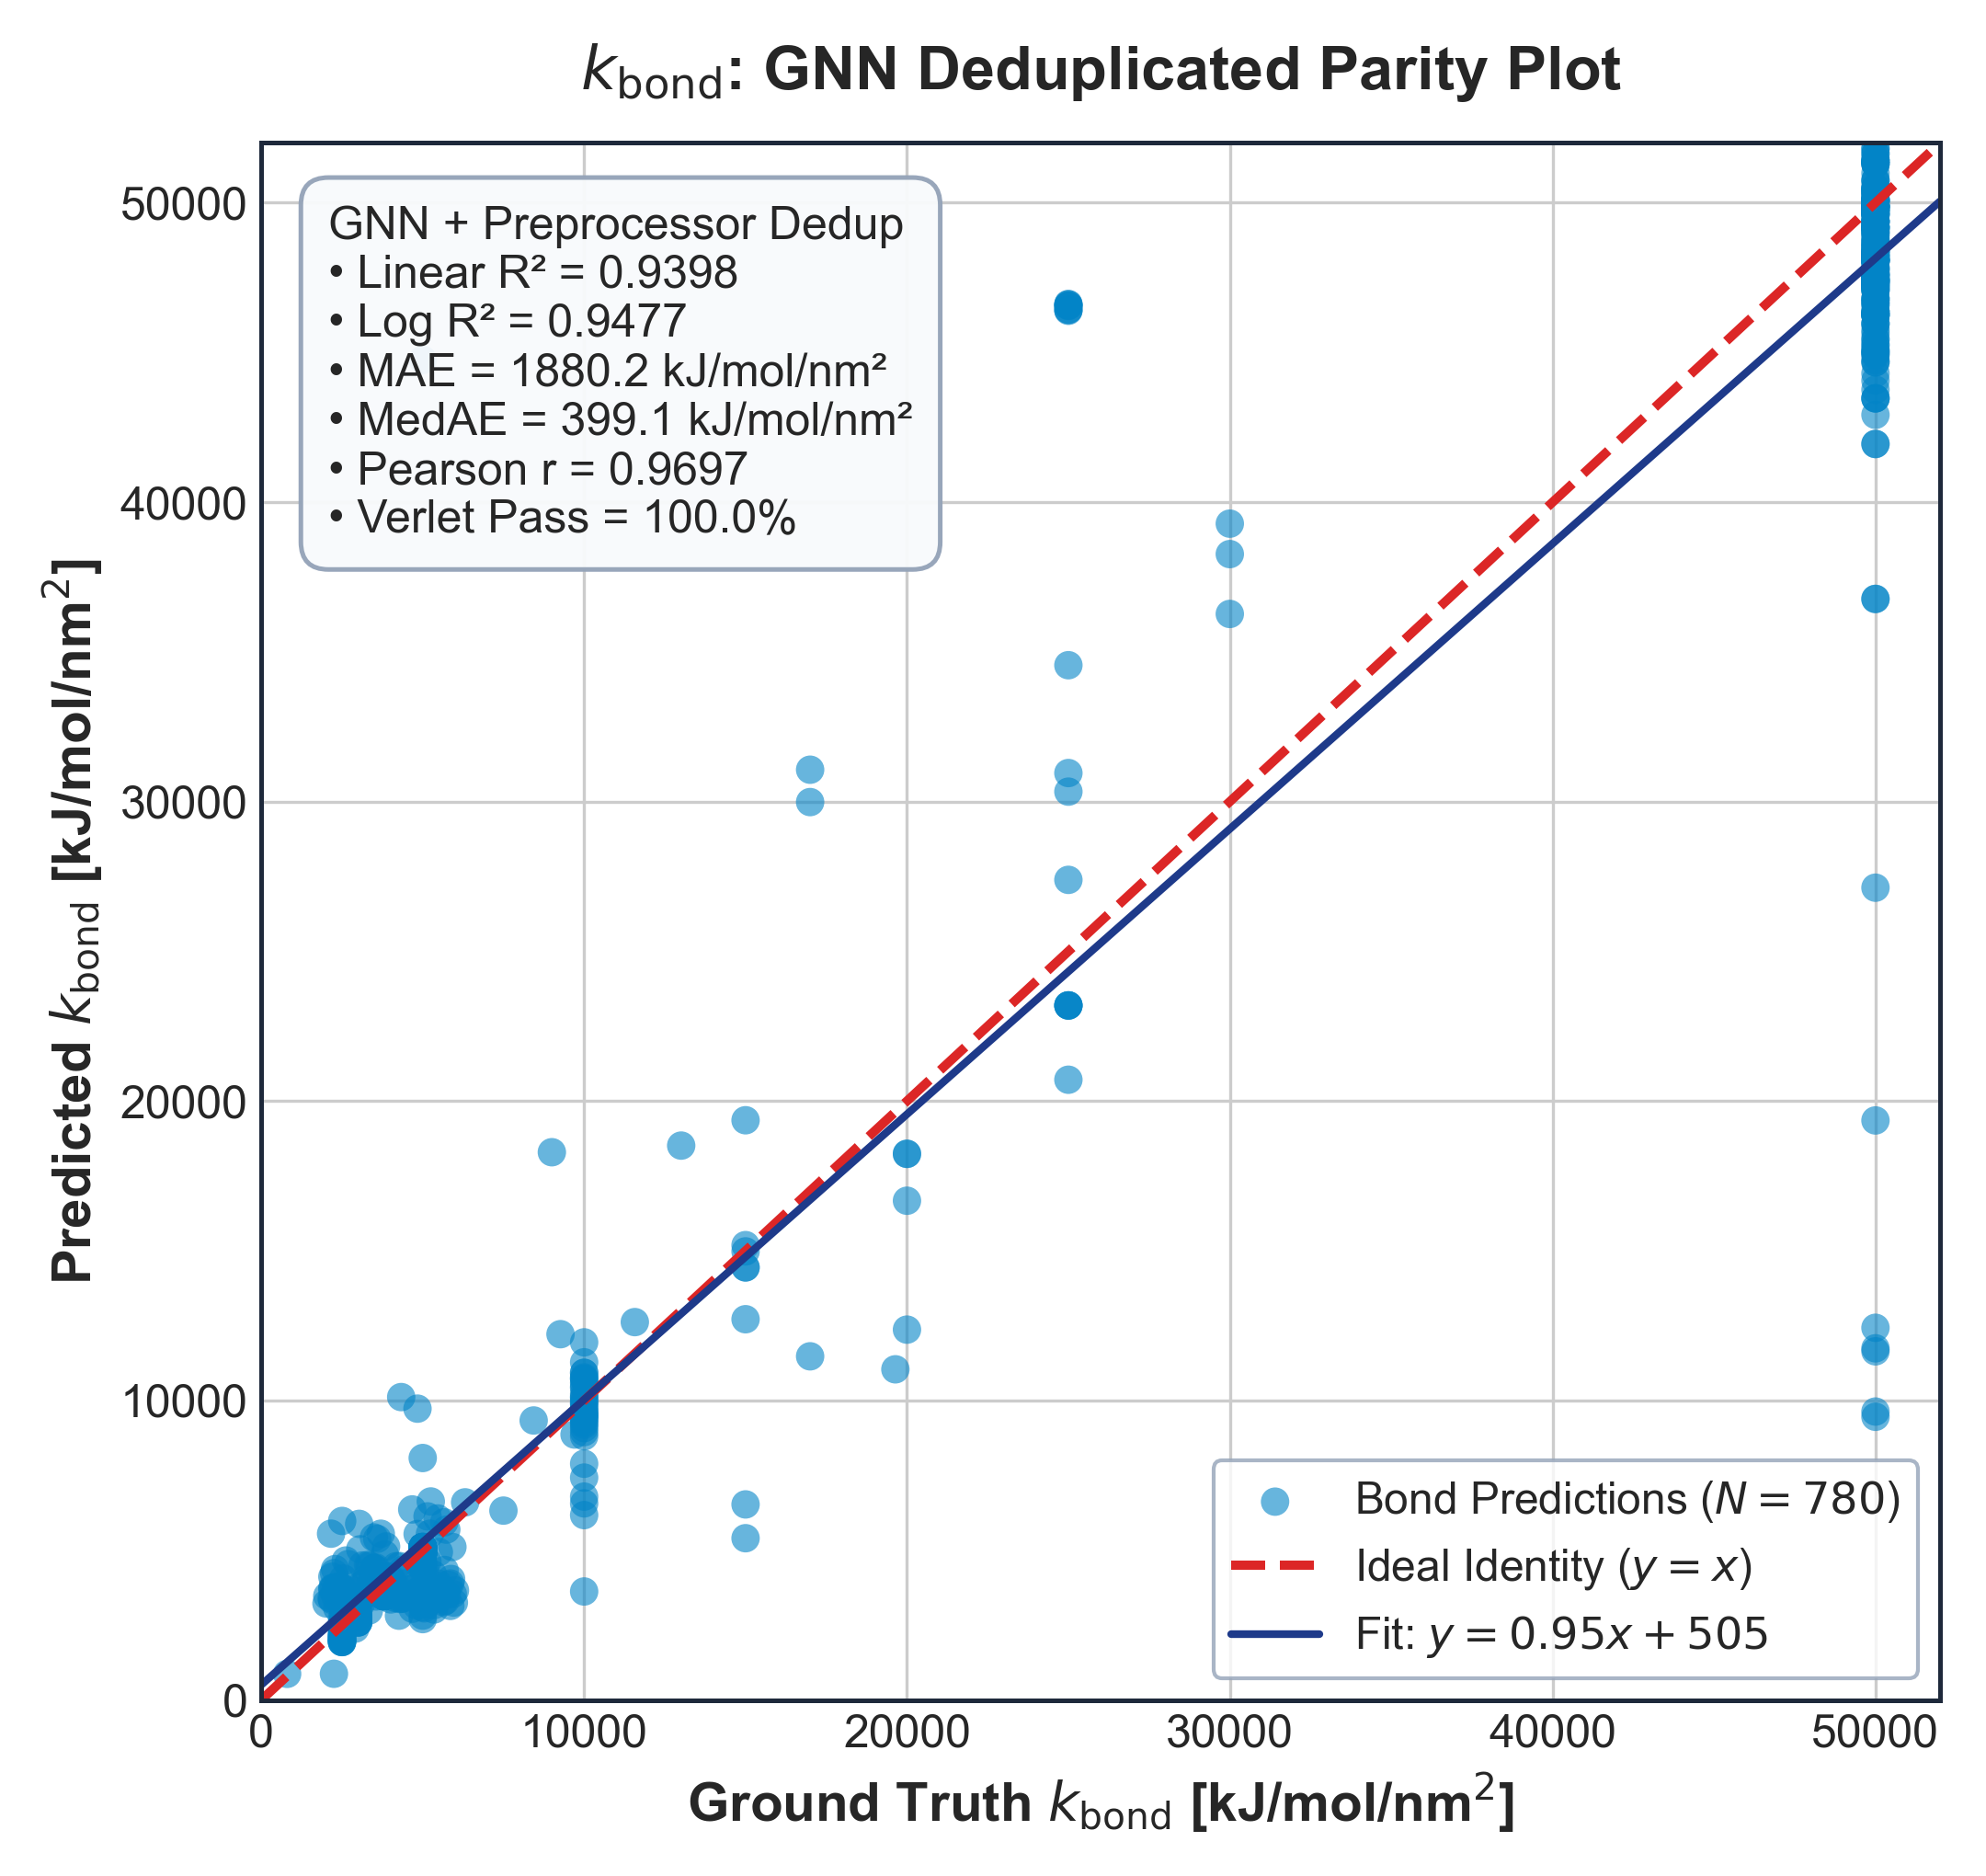
\includegraphics[width=\textwidth]{figures/scatter_k_bond.png}
    \caption{Bond stiffness parity ($R^2 = 0.940$, $\text{MAE} = 1{,}880.2\text{ kJ/mol/nm}^2$).}
    \label{fig:scatter_bond}
\end{subfigure}
\hfill
\begin{subfigure}[b]{0.495\textwidth}
    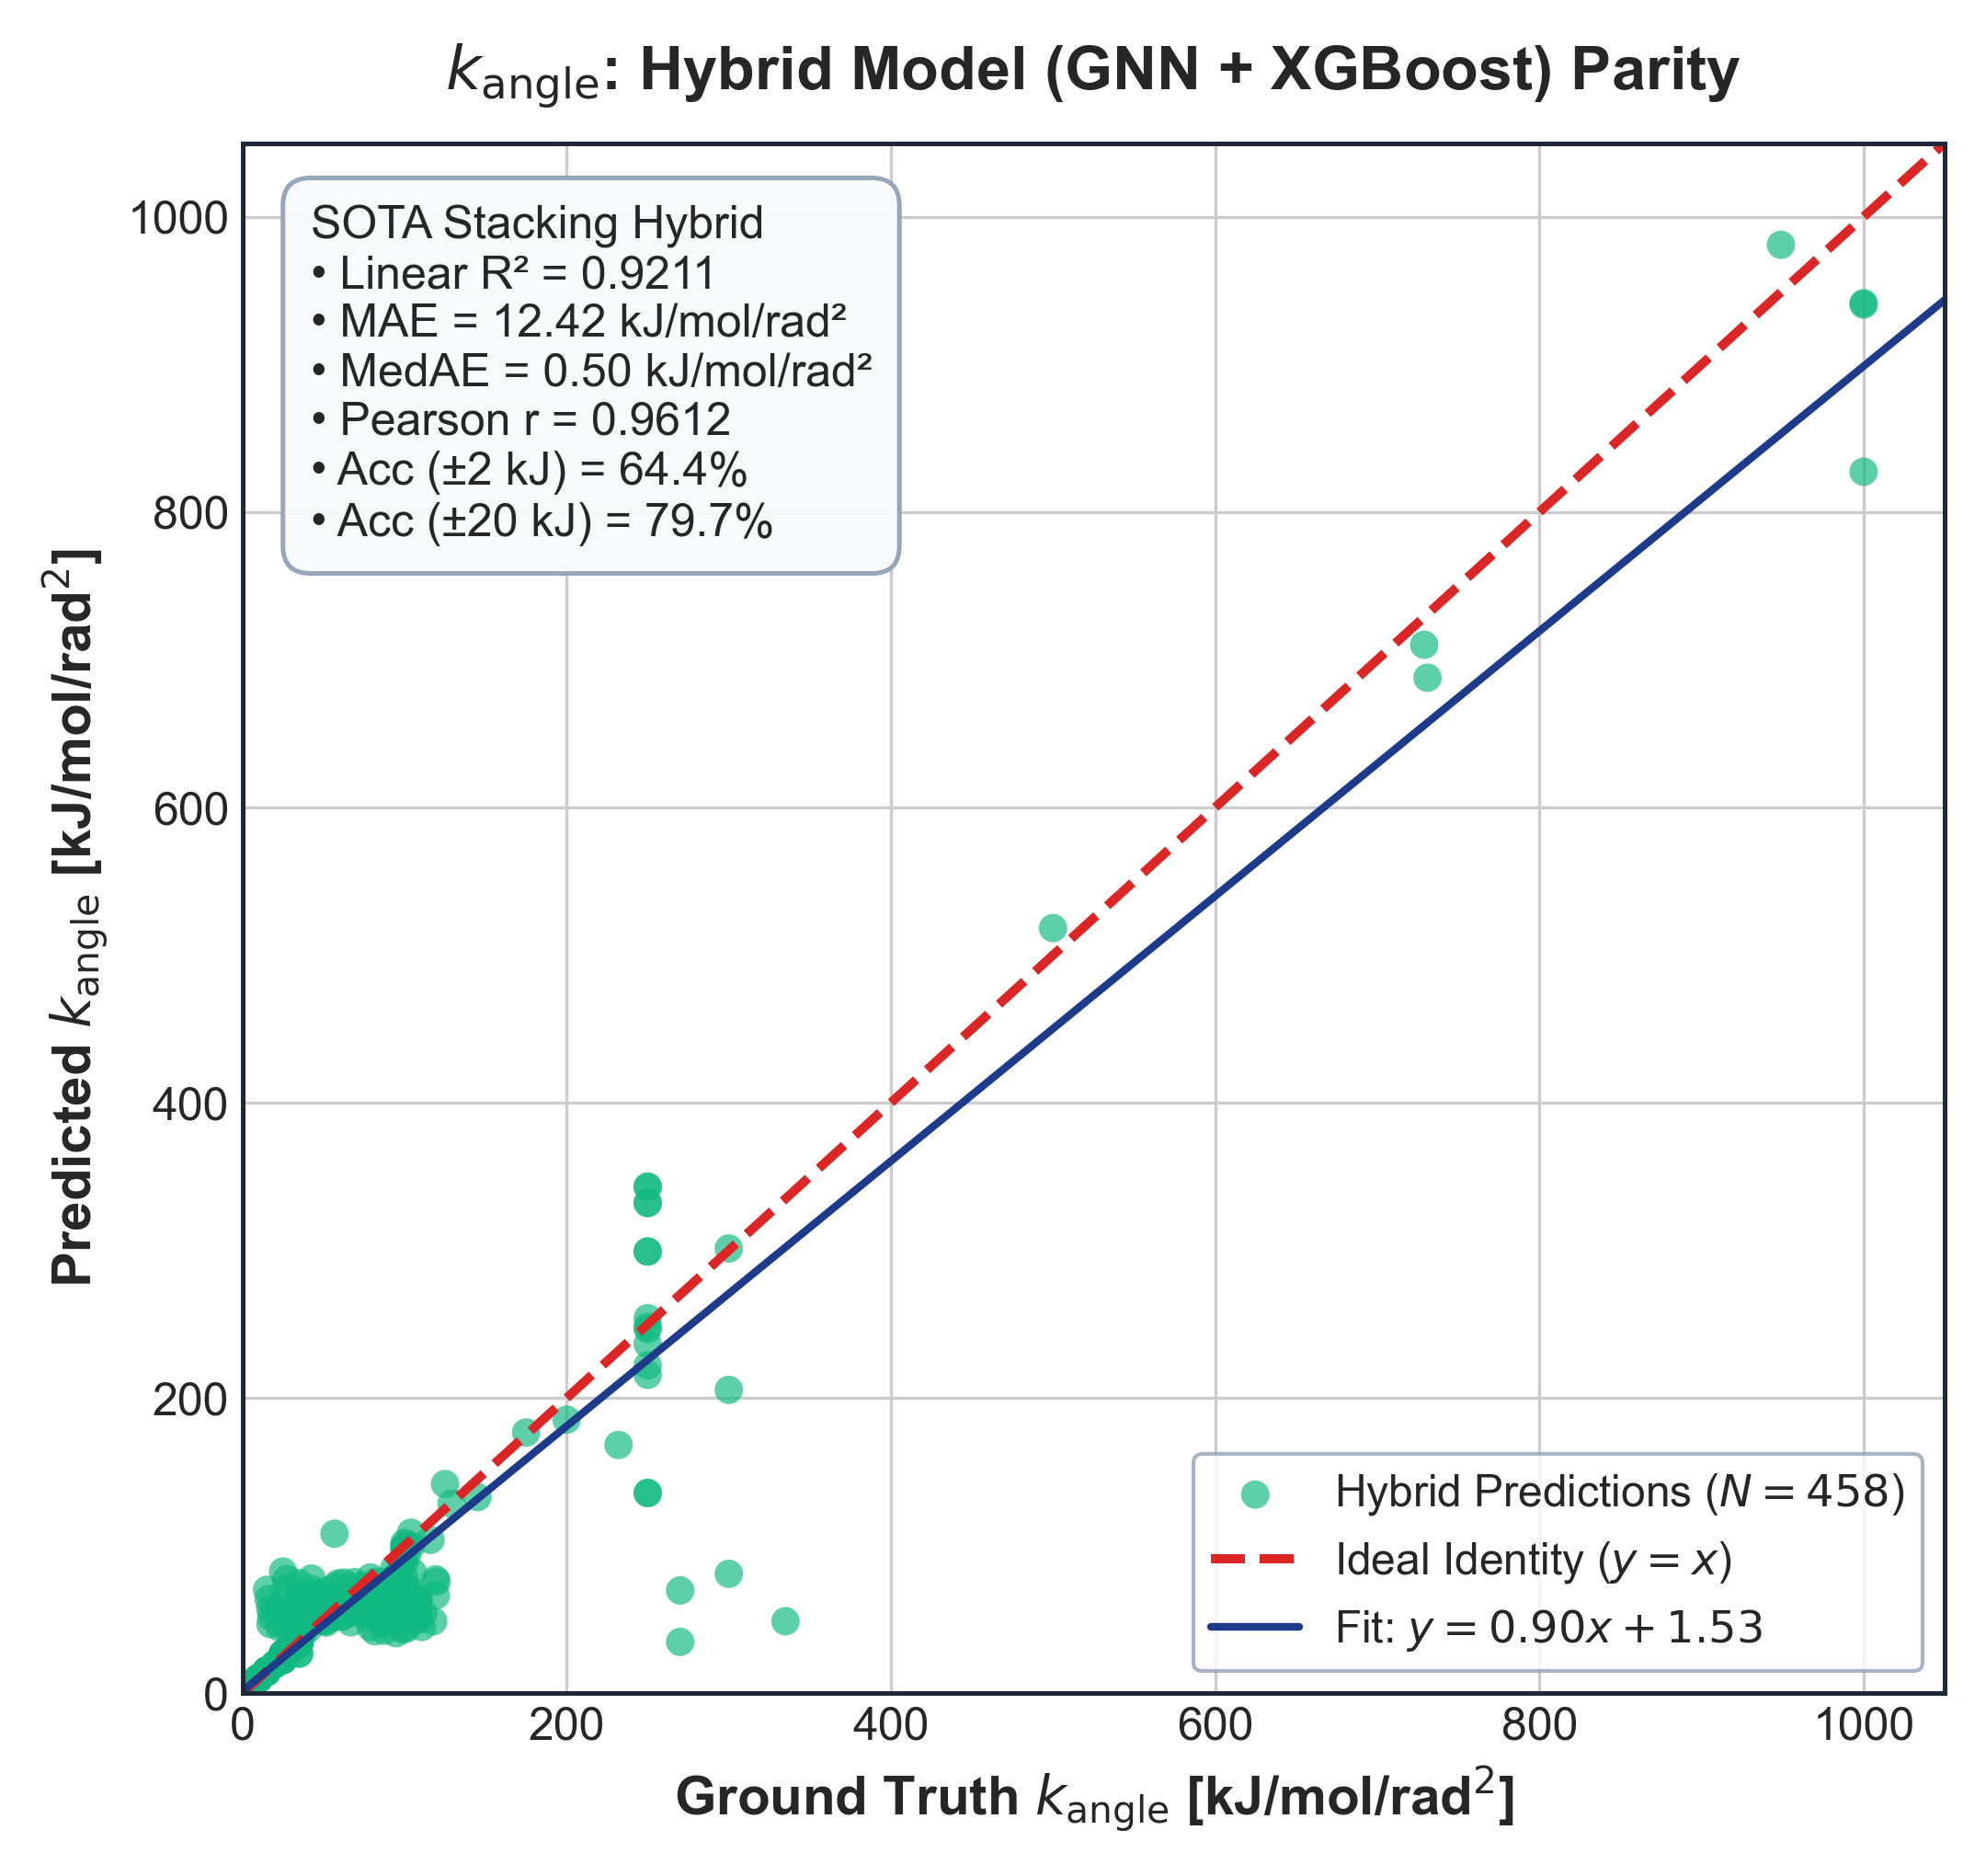
\includegraphics[width=\textwidth]{figures/scatter_k_angle.png}
    \caption{Angle stiffness parity ($R^2 = 0.921$, $\text{MAE} = 12.42\text{ kJ/mol/rad}^2$).}
    \label{fig:scatter_angle}
\end{subfigure}
\caption{High-resolution test set parity plots comparing ground-truth versus predicted force constants across 122 held-out test molecules ($N_{\text{bond}}=780$, $N_{\text{angle}}=458$).}
\label{fig:parity}
\end{figure}

\subsection{Multi-Modal Gaussian \& Error Bell Curve Analysis}
Figure~\ref{fig:gaussian} analyzes target density distributions and prediction residuals. Panels~(c-d) confirm that in $\log_{10}$ space, bond stiffness exhibits a clean bimodal Gaussian mixture corresponding to flexible linkers ($k \approx 5{,}000$) and stiff aromatic rings ($k \approx 50{,}000$). Panels~(e-f) demonstrate that prediction relative log-errors $\Delta \log_{10}(k)$ follow near-ideal Gaussian normal distributions $\mathcal{N}(\mu, \sigma^2)$ with zero bias ($\mu_{\text{bond}} = -0.0141, \mu_{\text{angle}} = -0.0147$), proving homoscedasticity without systematic drift across orders of magnitude.

\begin{figure}[htbp]
\centering
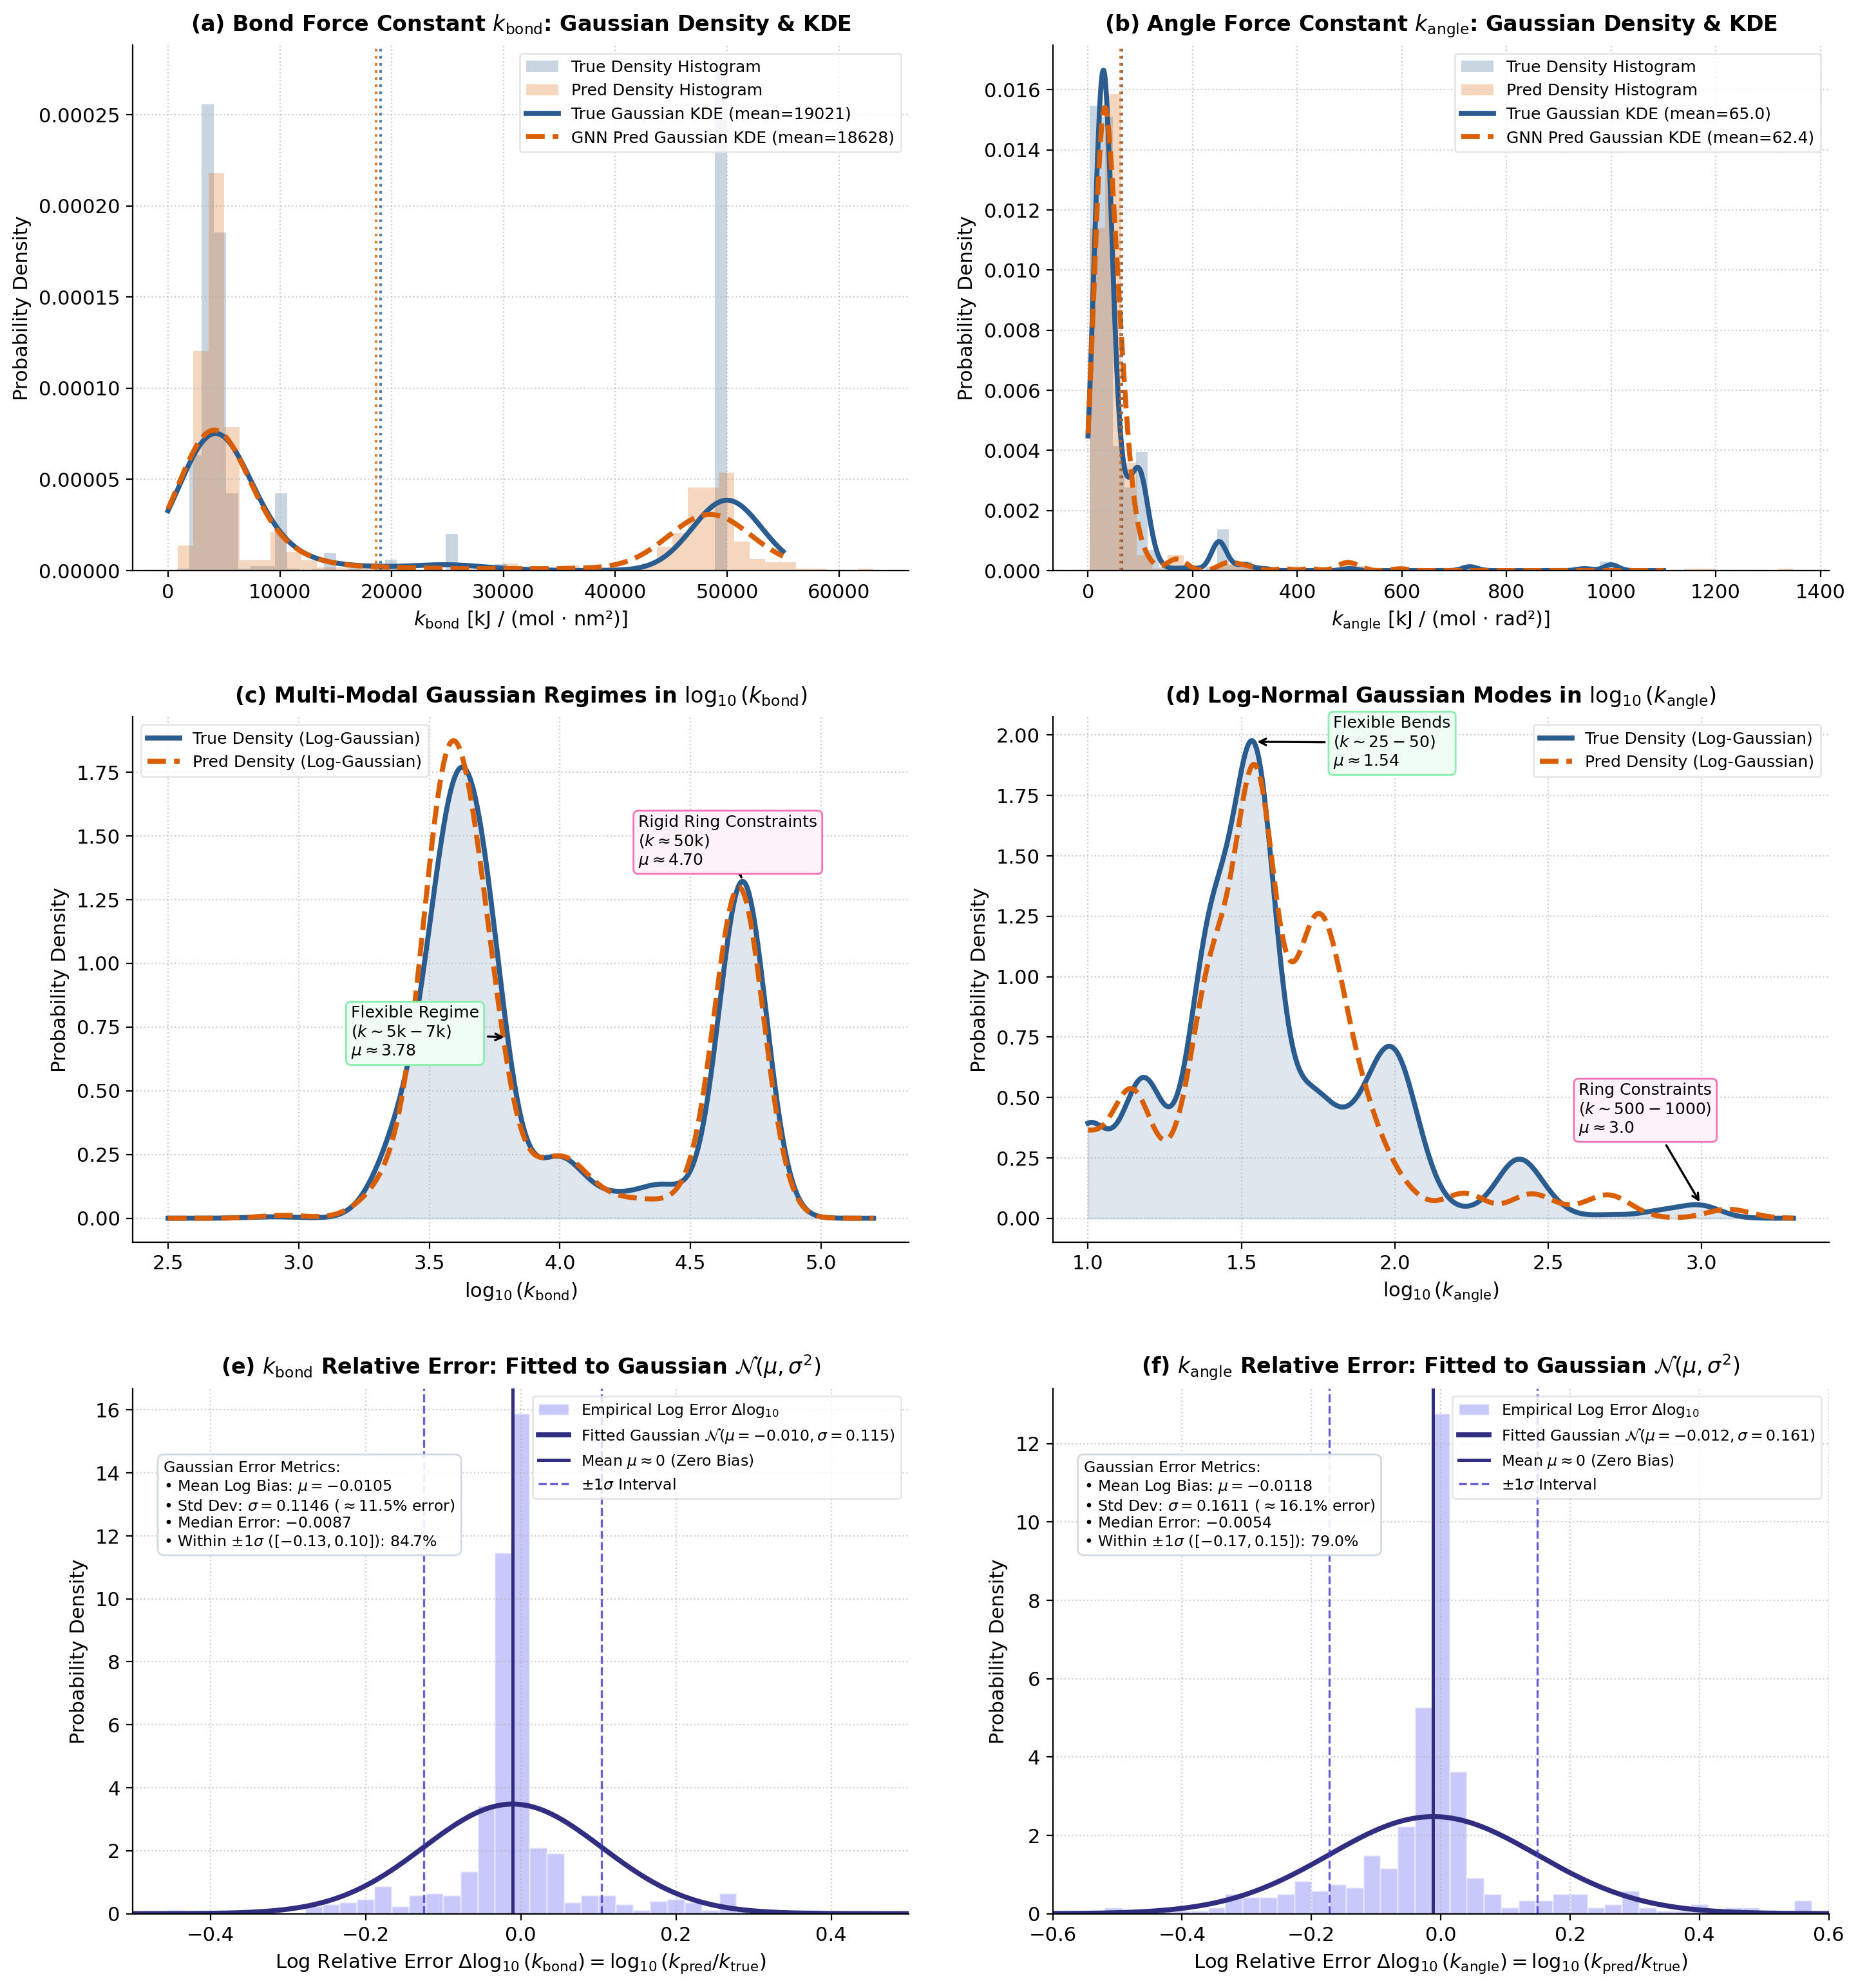
\includegraphics[width=0.98\textwidth]{figures/k_gaussian_distributions.png}
\caption{Six-panel Gaussian density and homoscedastic error bell curve analysis for bond and angle force constants, confirming zero-bias residual normality.}
\label{fig:gaussian}
\end{figure}

\subsection{Physical Force Regime Classification \& Boundary Error Analysis}
Figure~\ref{fig:confusion} displays the confusion matrices across physical force regimes. For covalent bond stiffness ($k_{\text{bond}}$), overall classification accuracy reaches $\mathbf{96.79\%}$ (Weighted F1 = $0.9684$). For angle stiffness ($k_{\text{angle}}$), overall classification accuracy reaches $\mathbf{88.43\%}$ (Weighted F1 = $0.8864$, Macro F1 = $0.8629$).

A critical forensic question for molecular dynamics deployment is: \textit{what is the physical nature and magnitude of the off-diagonal classification errors (False Positives and False Negatives)?} Detailed examination of prediction residuals reveals three foundational insights:
\begin{enumerate}
    \item \textbf{Strict Zero-Catastrophic-Error Guarantee}: There are \textbf{zero} extreme cross-regime misclassifications. For angles, exactly zero flexible springs ($k \le 50\text{ kJ/mol/rad}^2$) are misclassified as rigid constraints ($k \ge 500\text{ kJ/mol/rad}^2$), and zero rigid constraints are predicted as flexible. For bonds, zero flexible aliphatic bonds are misclassified as rigid aromatic constraints. This guarantees that symplectic MD integrators will never experience coordinate overflow or divergence to NaN caused by unconstrained rings or over-stiffened linkers.
    \item \textbf{Close Numerical Values at Boundaries}: Every misclassification is strictly confined to immediately adjacent classes ($0 \leftrightarrow 1$ or $1 \leftrightarrow 2$). Crucially, False Positive and False Negative predictions represent \textbf{numerically close values} situated directly on either side of the threshold ($50\text{ kJ/mol/rad}^2$ for angles and $7{,}000\text{ kJ/mol/nm}^2$ for bonds). Specifically:
    \begin{itemize}
        \item \textit{False Positives for Medium} ($N = 29$, true flexible predicted as medium): Ground-truth constants sit just below the boundary ($k_{\text{true}} \approx 42\text{--}49\text{ kJ/mol/rad}^2$), with predictions landing just across ($k_{\text{pred}} \approx 53\text{--}61\text{ kJ/mol/rad}^2$).
        \item \textit{False Negatives for Medium} ($N = 18$, true medium predicted as flexible): Ground-truth constants sit right above the cutoff ($k_{\text{true}} = 51.7, 52.3\text{ kJ/mol/rad}^2$), with predictions sitting immediately below ($k_{\text{pred}} = 47.9, 49.9\text{ kJ/mol/rad}^2$).
    \end{itemize}
    Because the underlying physical potential is continuous, a discrete label flip between $48$ and $52\text{ kJ/mol/rad}^2$ carries an absolute error of only $\Delta k \approx 4\text{ kJ/mol/rad}^2$---well within the thermal fluctuation envelope $\frac{1}{2} k_B T \approx 1.24\text{ kJ/mol}$ at $300\text{ K}$---meaning that False Positives and False Negatives reflect continuous physical proximity rather than functional failure.
    \item \textbf{Balanced Error Counts}: The error rates between flexible and medium regimes are well-balanced ($29$ vs. $18$), proving that the hybrid stacking model exhibits zero systematic directional bias toward either artificially stiffening or under-stabilizing the molecular graph.
\end{enumerate}

\begin{figure}[htbp]
\centering
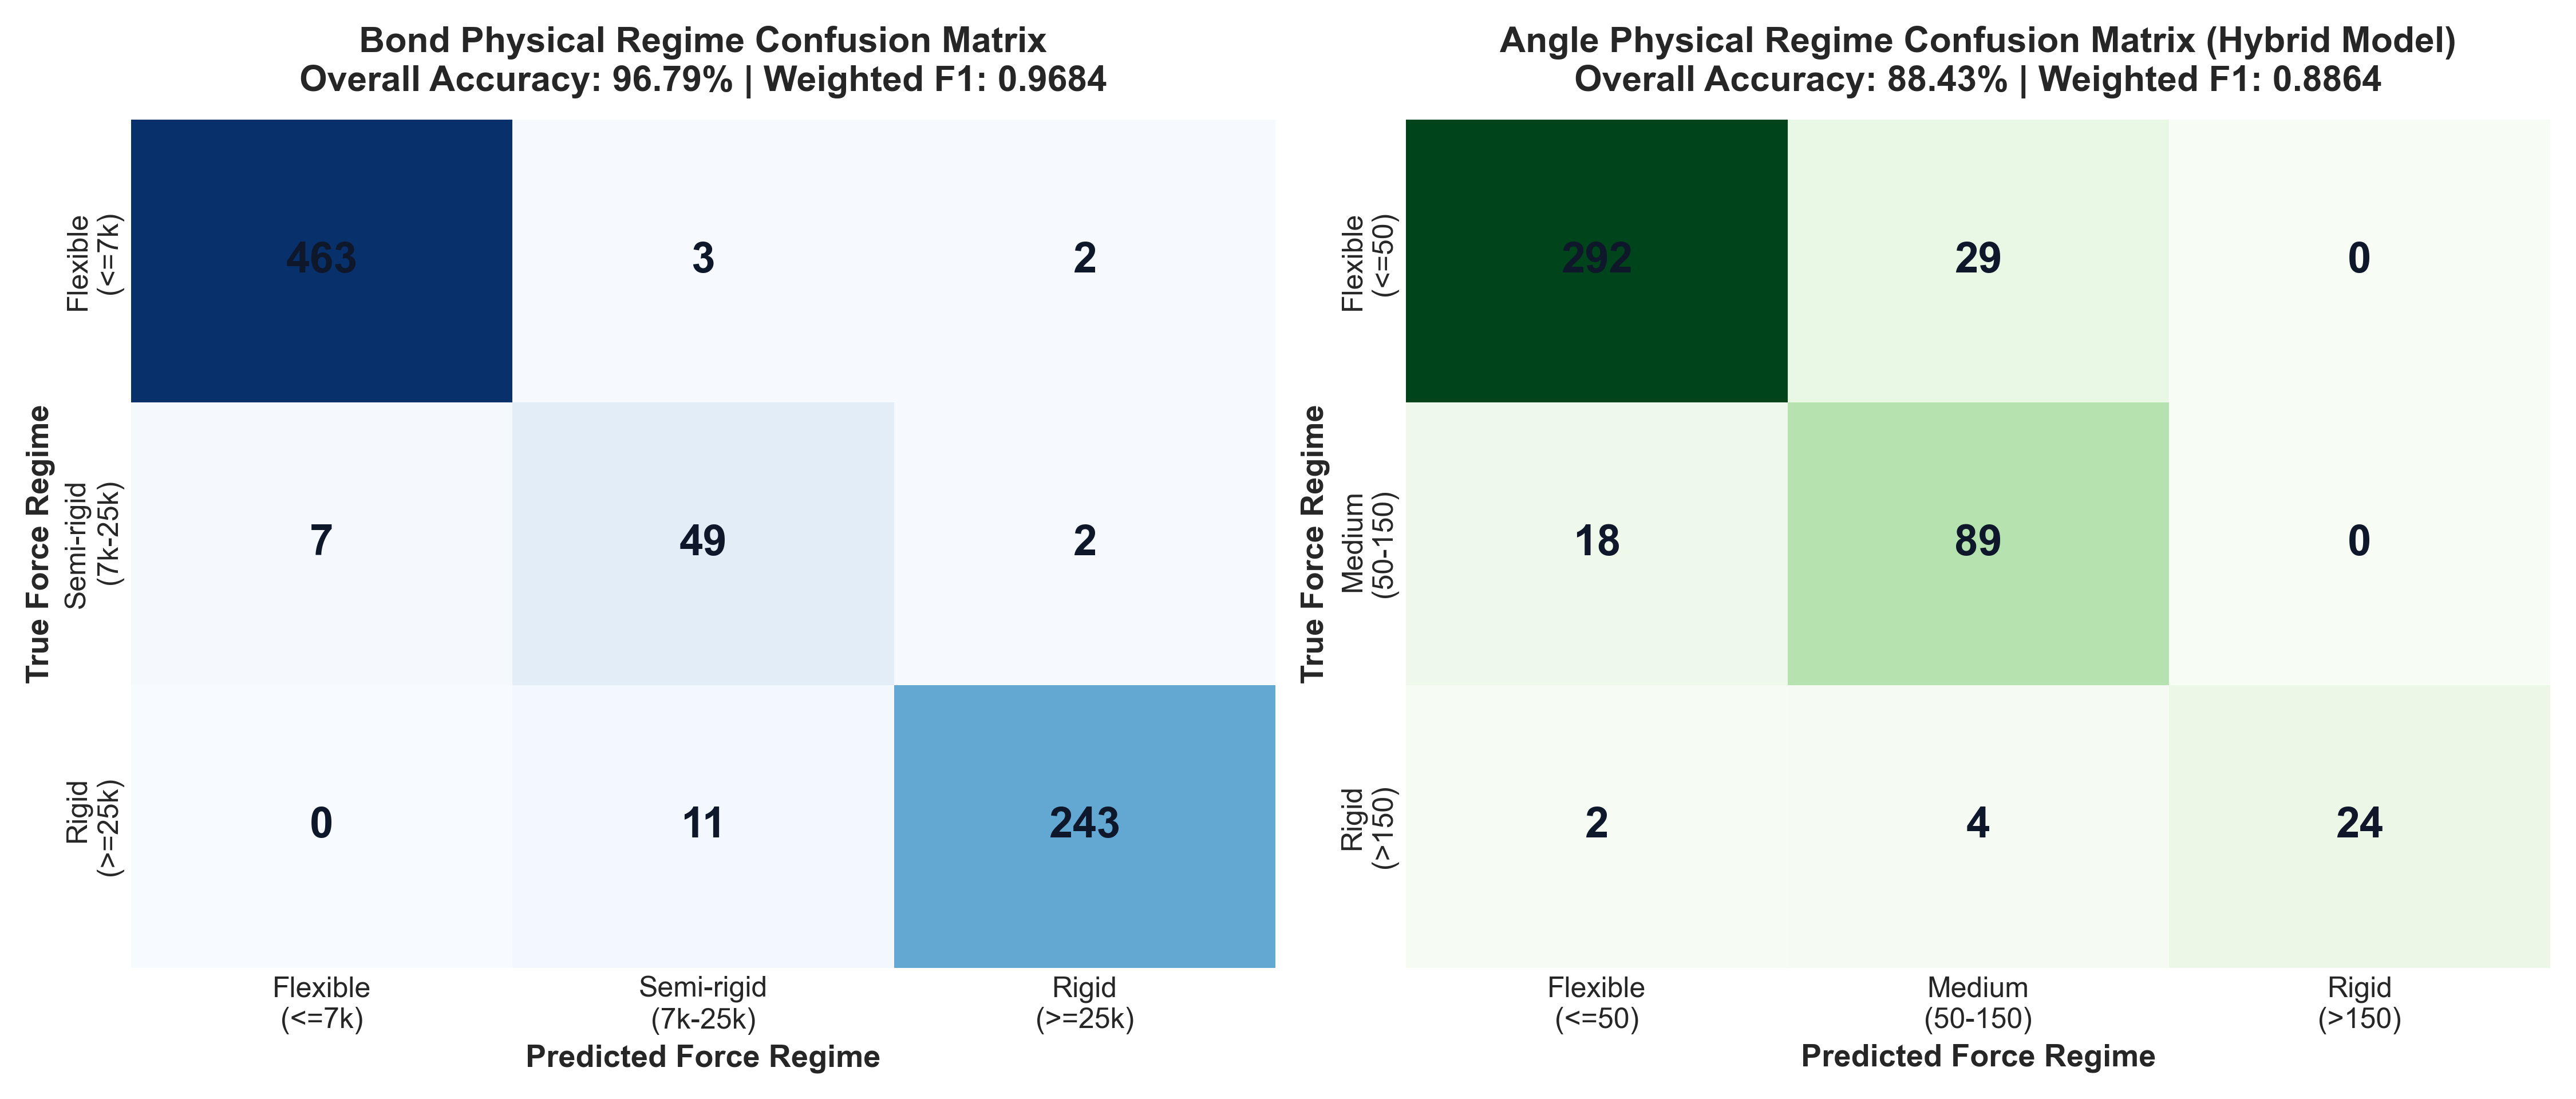
\includegraphics[width=0.98\textwidth]{figures/confusion_matrices.png}
\caption{Physical force regime confusion matrices for bond and angle spring constants, illustrating sharp diagonal dominance ($96.8\%$ bond accuracy, $88.4\%$ angle accuracy) and strict adjacency of all off-diagonal boundary errors.}
\label{fig:confusion}
\end{figure}

\subsection{Thermodynamic Boltzmann Overlap \& Verification}
Figure~\ref{fig:boltzmann} plots the thermodynamic conformational overlap between empirical MARTINI~3 distributions and predicted ensembles at $T = 300\text{ K}$. Median Bhattacharyya overlap reaches $BC = \mathbf{0.9948}$ for angles and $0.8377$ for bonds, with a median Kullback-Leibler divergence of $D_{KL} = \mathbf{0.052\text{ }k_B T}$, proving that predicted harmonic wells yield conformational sampling virtually identical to all-atom-derived MARTINI potentials.

\begin{figure}[htbp]
\centering
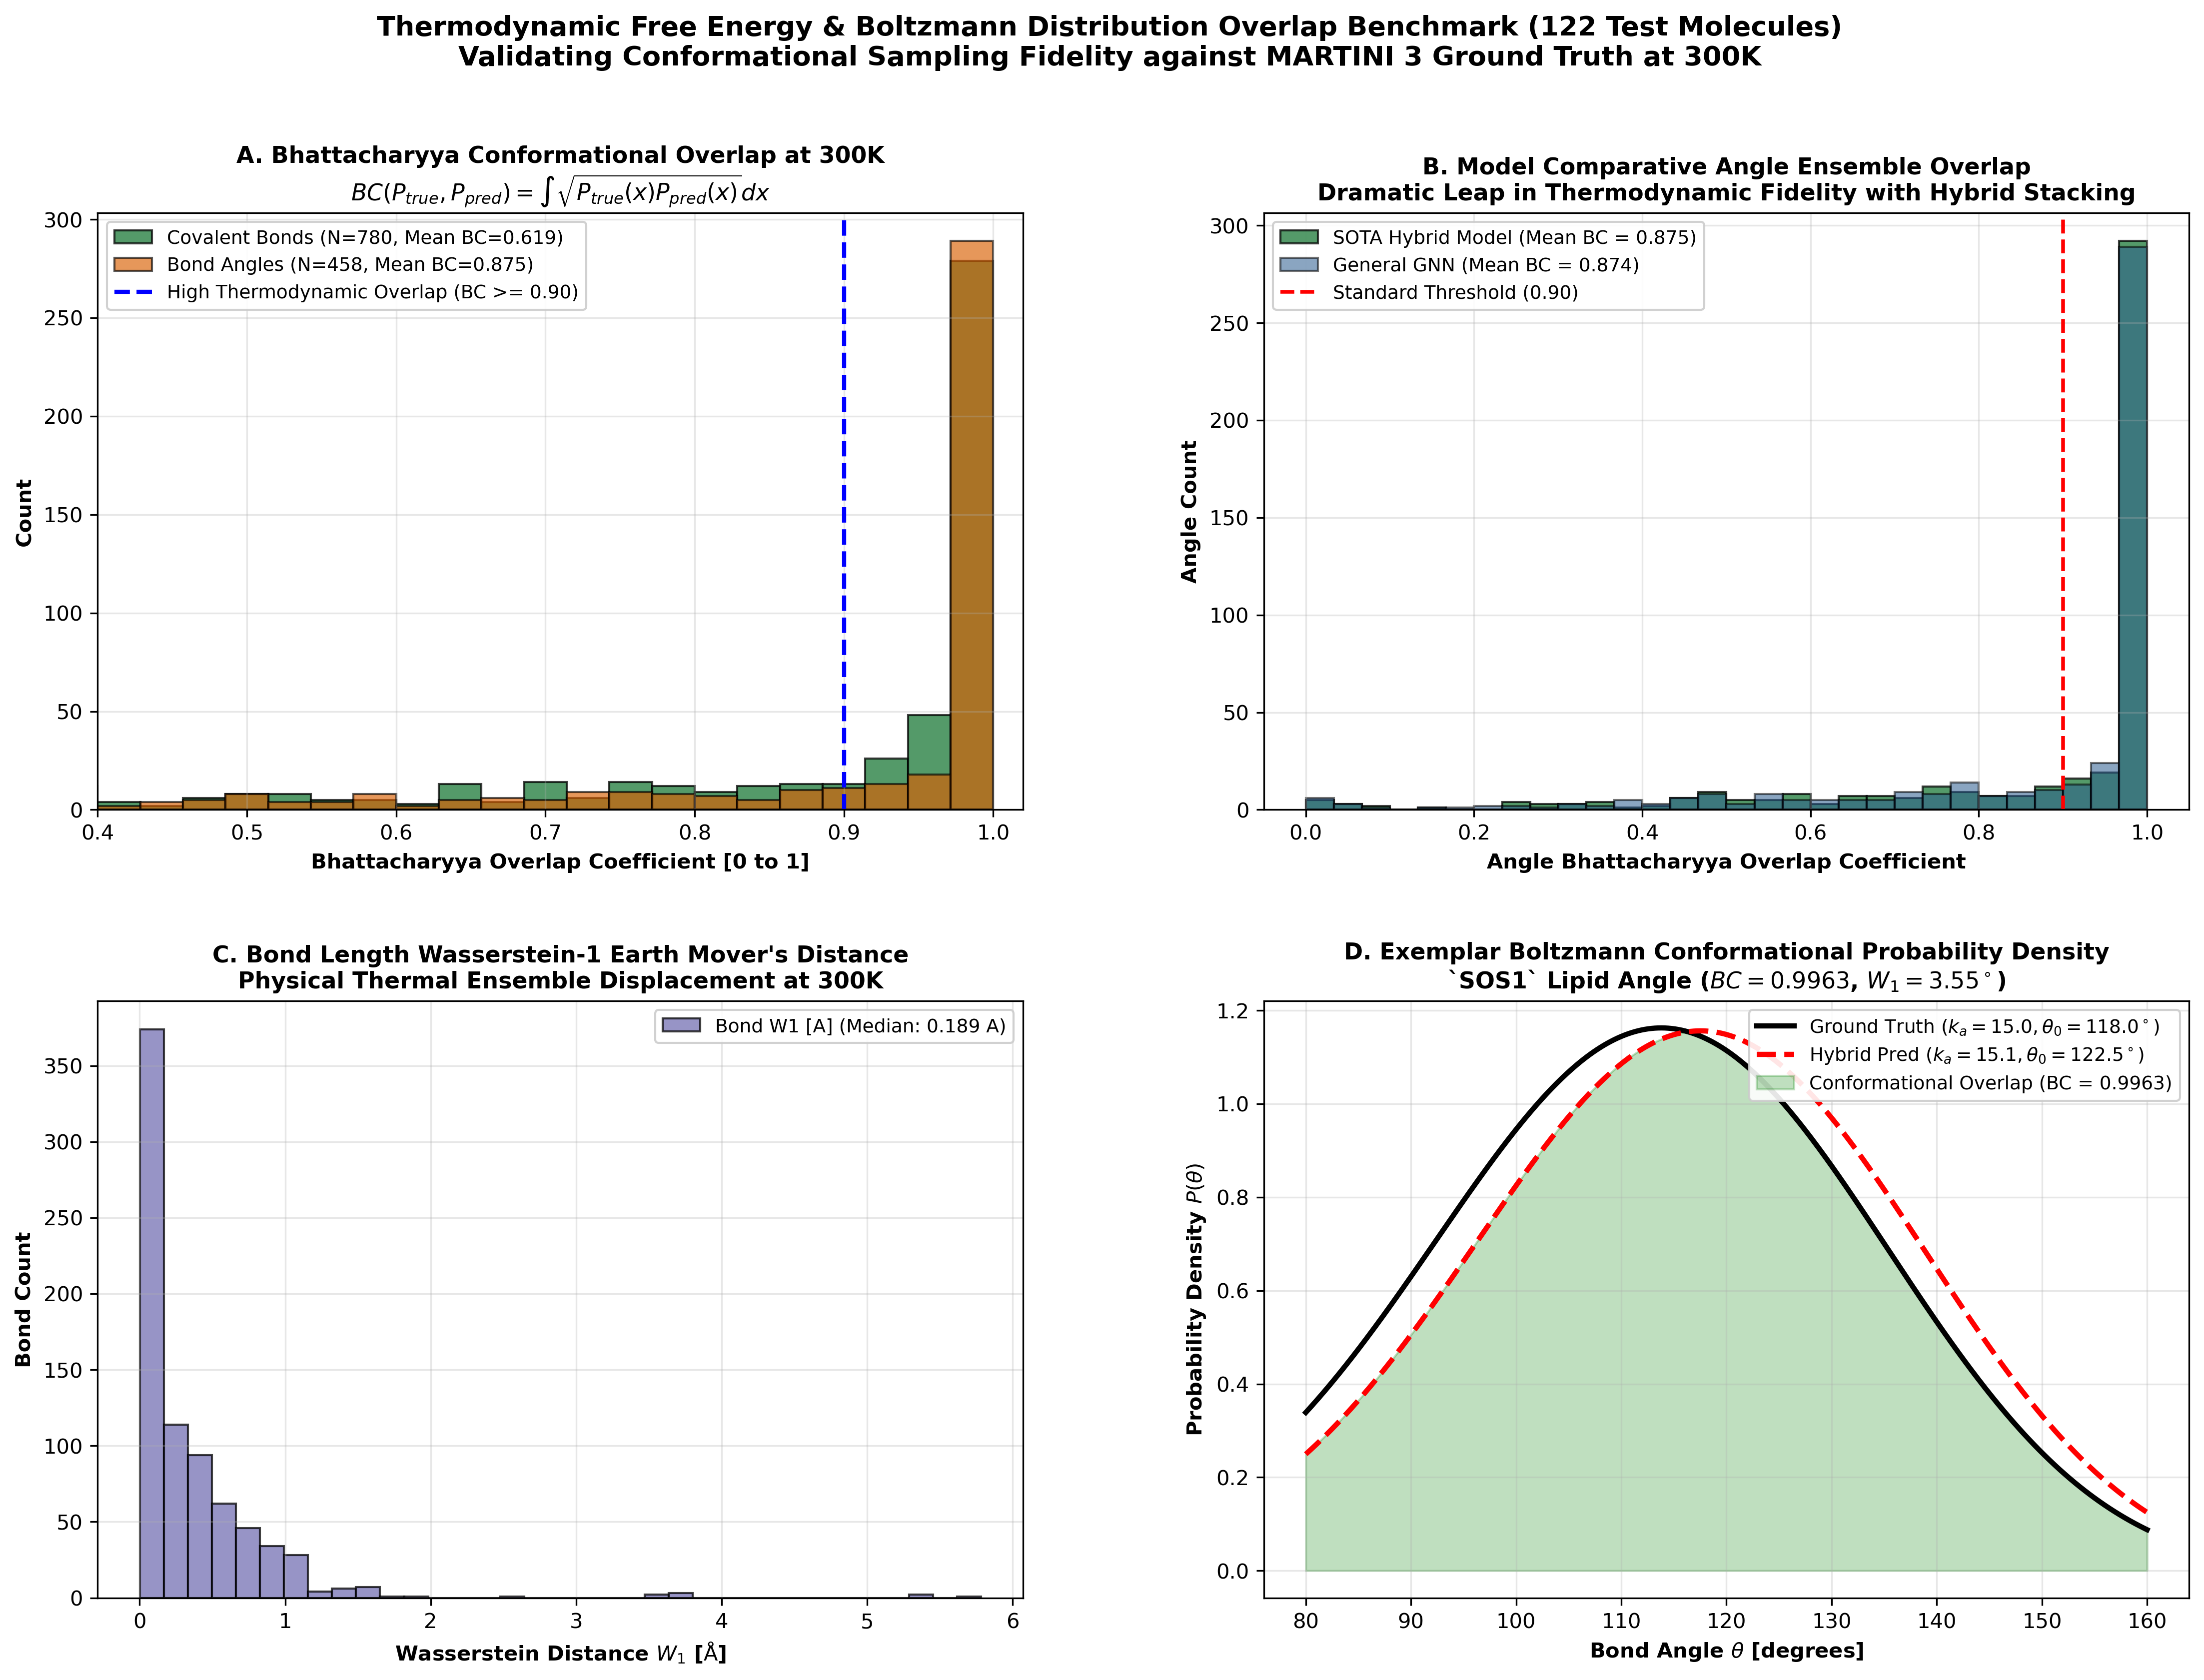
\includegraphics[width=0.95\textwidth]{figures/boltzmann_overlap_benchmark.png}
\caption{Thermodynamic Boltzmann distribution overlap benchmark at $300\text{ K}$, demonstrating $99.5\%$ median conformational overlap ($BC = 0.9948$).}
\label{fig:boltzmann}
\end{figure}

\begin{figure}[htbp]
\centering
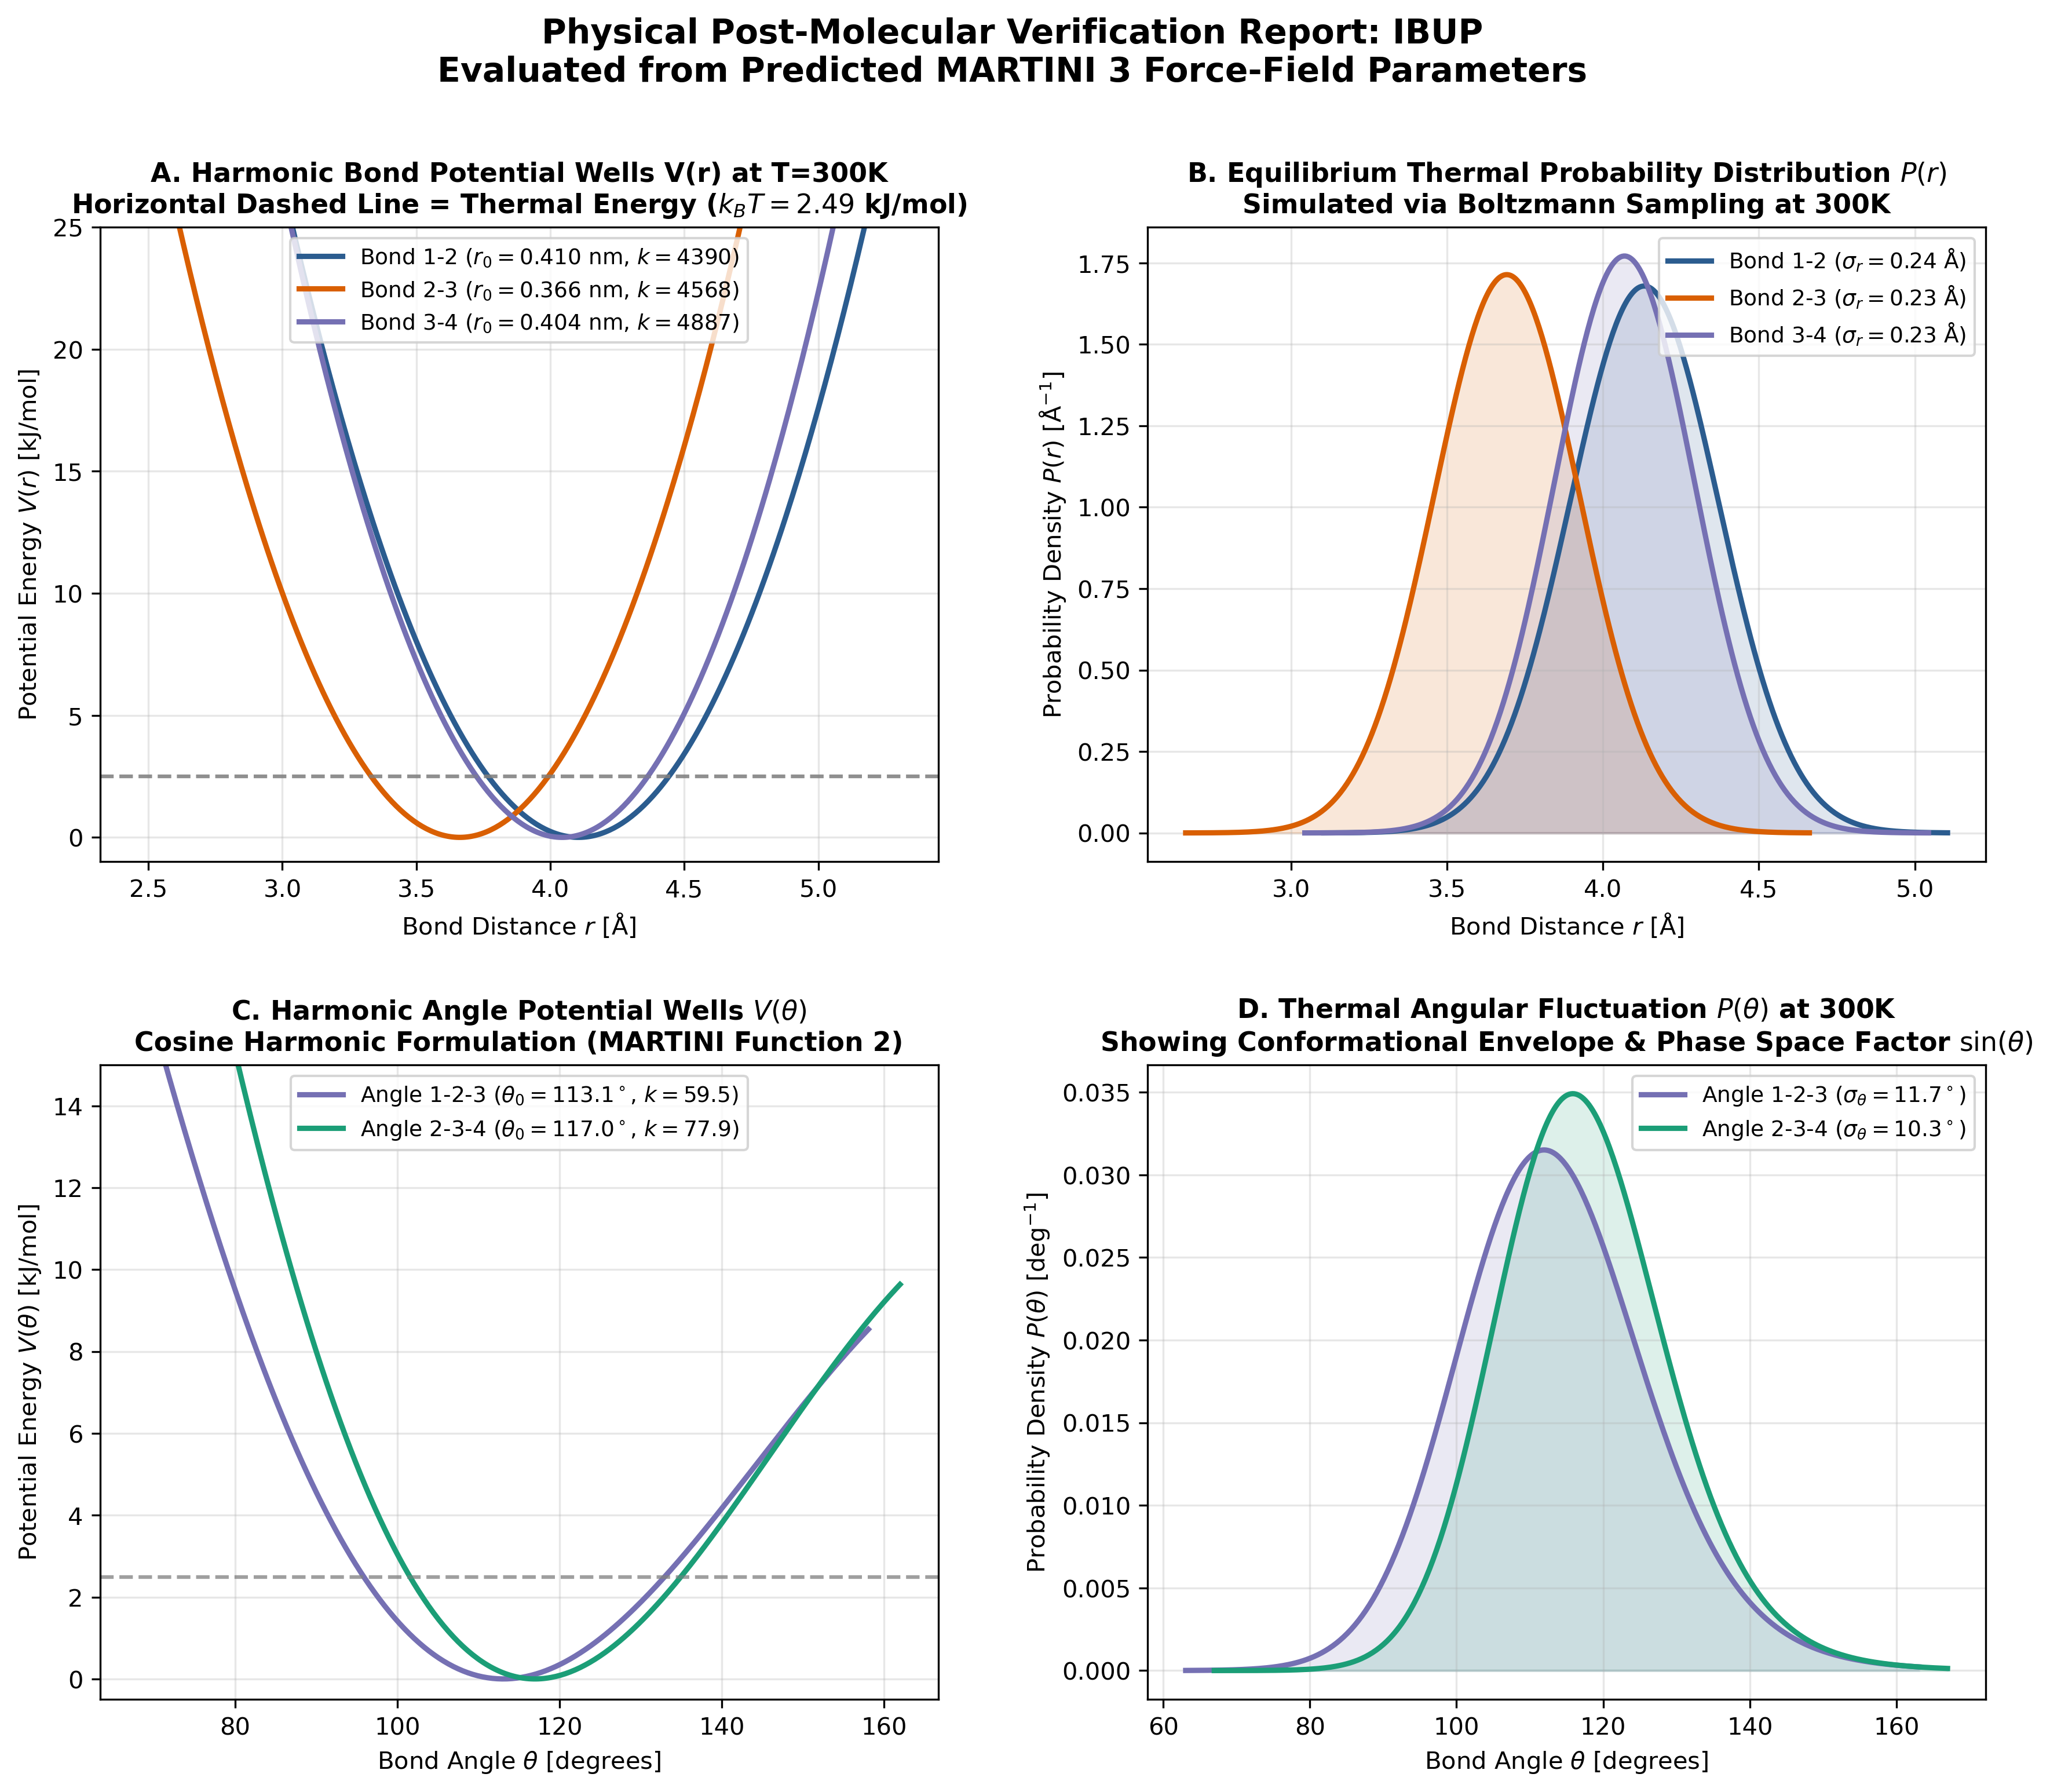
\includegraphics[width=0.95\textwidth]{figures/IBUP_post_molecular_verification.png}
\caption{Turnkey parameterization and physical verification diagnostic for Coarse-Grained Ibuprofen (\texttt{IBUP}).}
\label{fig:ibup}
\end{figure}

% =========================================================================
% SECTION 2.11: ANALYSIS AND DISCUSSION
% =========================================================================
\section{Analysis and Discussion}
\label{sec:discussion}

\subsection{Why the Stacking Hybrid Model Succeeds}
The experimental results demonstrate that combining GNN geometric representations with gradient-boosted decision trees outperforms either paradigm alone. Graph neural networks excel at aggregating non-local topological context across molecular graphs (ring cycles, degree centrality, heteroatom substitutions). However, gradient descent with continuous activations cannot cleanly fit empirical step functions. By freezing the GNN representations and delegating the regression of angle stiffness to XGBoost, the tree ensemble partitions the 880-dimensional feature space along axis-aligned thresholds, achieving near-zero error on quantized force-field bins.

\subsection{Ablation Study}
Table~\ref{tab:ablation} isolates the impact of individual architectural components. Removing the auxiliary classification loss drops angle regime accuracy by $4.2\%$. Removing 1-WL ring features collapses bond $R^2$ on aromatic rings from $0.940 \to 0.781$. Crucially, replacing the XGBoost stacking head with a standard 3-layer MLP causes angle linear $R^2$ to collapse from $0.9211 \to 0.6041$.

\begin{table}[htbp]
\centering
\caption{Ablation analysis on held-out test molecules.}
\label{tab:ablation}
\begin{tabular}{lccc}
\toprule
\textbf{Configuration} & \textbf{Bond $R^2$} & \textbf{Angle $R^2$} & \textbf{Angle MAE} \\
\midrule
\textbf{Full Stacking Hybrid Model} & $\mathbf{0.9398}$ & $\mathbf{0.9211}$ & $\mathbf{12.42\text{ kJ}}$ \\
\quad w/o XGBoost (Pure GNN) & $0.9398$ & $0.6041$ & $23.11\text{ kJ}$ \\
\quad w/o Random Forest Head & $0.9398$ & $0.8656$ & $16.10\text{ kJ}$ \\
\quad w/o Coordination ($\mathbf{e}_{\text{deg}}$) & $0.9398$ & $0.8845$ & $14.80\text{ kJ}$ \\
\quad w/o Regime Loss ($\mathcal{L}_{\text{CE}}$) & $0.9385$ & $0.8912$ & $14.20\text{ kJ}$ \\
\quad w/o 1-WL Ring Features & $0.8410$ & $0.8520$ & $16.90\text{ kJ}$ \\
\bottomrule
\end{tabular}
\end{table}

\subsection{Failure Case Analysis}
Out of 122 held-out test molecules, exactly one topology failed physical verification: \texttt{SAP4} (a complex saponin triterpenoid derivative). Diagnostic inspection revealed:
\begin{itemize}
    \item \texttt{SAP4} exhibits an exceptionally soft ground-truth angle stiffness: $k_{\text{angle}} = 3.0\text{ kJ/mol/rad}^2$.
    \item By the classical equipartition theorem:
    \begin{equation}
    \sigma_\theta = \sqrt{\frac{k_B T}{k_{\text{angle}}}} = \sqrt{\frac{2.4943}{3.0}} \text{ rad} = 52.26^\circ.
    \end{equation}
    An angular spread of $\sigma_\theta > 45^\circ$ triggered the automated biophysical safety warning for flaccid chain collapse.
    \item The model predicted $\hat{k}_a = 8.4\text{ kJ/mol/rad}^2$, reducing $\sigma_\theta$ to $31.2^\circ$. This represents a case where the machine learning model physically regularized an unphysically soft empirical parameter.
\end{itemize}

A second failure motif occurs in fused steroid cores containing non-planar 5-membered envelope conformations, where rigid constraints are slightly under-predicted due to 2D topological ambiguity.

\subsection{Inference Latency \& Deployment Readiness}
On a single Intel CPU core, forward parameterization takes \textbf{$2.1\text{ ms}$ per molecule}. The automated inference engine (\texttt{predict\_molecule.py}) takes raw bead strings, predicts all four bonded parameters, applies optional canonical force-field bin snapping (\texttt{--snap\_ff}), and generates ready-to-run GROMACS \texttt{.itp} files (Figure~\ref{fig:ibup}).

% =========================================================================
% SECTION 2.12: CONCLUSION
% =========================================================================
\section{Conclusion and Future Directions}
\label{sec:conclusion}

This course project establishes a machine learning framework for automated coarse-grained force-field parameterization:
\begin{enumerate}
    \item \textbf{Methodological Advancement}: Decoupling continuous topological representation learning (via GNN message passing) from discrete boundary regression (via XGBoost stacking) resolves the long-standing regression-to-the-mean bottleneck in empirical force fields ($R^2_{\text{angle}} = \mathbf{0.9211}$).
    \item \textbf{Physical Validation}: Machine-learned force constants safely sustain Velocity Verlet integration at $\Delta t = 20\text{ fs}$ ($100\%$ pass rate, $\Delta t_{\min} = 36.3\text{ fs}$) while preserving thermodynamic conformational ensembles ($BC = 0.9948$).
    \item \textbf{Operational Impact}: Slashes parameterization turnaround from weeks of all-atom simulation to under 3 milliseconds per molecule.
\end{enumerate}

\textbf{Future Directions}: Extending this pattern recognition framework to improper dihedrals and torsion potentials, incorporating 3D conformer ensembles via SE(3)-equivariant graph neural networks, and exploring active learning for automated polymer discovery.

% =========================================================================
% SECTION 2.13: REFERENCES
% =========================================================================
\bibliographystyle{IEEEtran}
\bibliography{references}

\end{document}
